\section{abstract}
Diagnostic ultrasound has been shown to cause lung hemorrhage in a
variety of mammals, though the underlying damage mechanisms are still
unclear. Motivated by this problem, we use numerical simulations to
investigate the interaction of an ultrasound wave with the tissue-air
interface. A half positive cycle represented by a trapezoidal waveform
in tissue (modelled as water) impinges upon the lung (modelled as
air); to represent the rough surface of the lung, the interface
includes a small single-mode perturbation. We hypothesize that
ultrasound waves deposit sufficient baroclinic vorticity to drive the
growth of perturbations at water-air interfaces. Our simulations show
that the perturbation amplitude grows to sizes many times larger than
the original value, \emph{well after the wave has passed}. We
demonstrate that conventional (linear) acoustics cannot account for
such deformations. Instead, the perturbation growth is driven by
nonlinear effects, i.e., the baroclinic vorticity deposited along the
interface, due to the misalignment of the pressure gradient (acoustic
wave) and the density gradient (perturbed gas-liquid
interface). Despite its low amplitude, the acoustic wave deposits
sufficient vorticity because of the sharp density gradient. Based on
dimensional scaling analysis we demonstrate that the amplitude of the
interface grows as $t^{3/5}$ and scales with the circulation density
for cases in which the circulation is relatively constant after the
passage of the wave. Furthermore, we demonstrate that the linear
circulation density decreases as $t^{1/2}$ in certain regimes. Since
the configuration is heavy-to-light, the perturbation undergoes phase
inversion. If the interval between the pressure increase and decrease
is sufficient, both deposit vorticity of the same sign, which enhances
the perturbation growth. Conversely, if the interval is too short, the
vorticity deposited by the pressure increase is canceled by the
decrease. A further consequence is that one may be able to control the
growth of such perturbed interfaces by modulated the ultrasound wave.

\section{Introduction}%
\label{sec:introduction}%
\ac{DUS} is one of the safest forms of medical imaging and has become
ubiquitous in clinical practice. However it has been demonstrated to
cause \ac{LH} in a variety of mammals. While the problem does not
appear to be one of medical concern under typical clinical conditions,
the underlying physical mechanism is not well understood and more
information is needed. 

Over the last few decades \ac{DUS}-induced \ac{LH} has been studied
extensively and is the only known bioeffect of non-contrast, pulsed
\ac{US} known to occur in mammals under clinically relevant
conditions. While it has been not been directly demonstrated in
humans, it has been shown to occur in a variety of mammals including
mice, rats, rabbits, pigs, and monkeys
\citep{Child1990,OBrien2006a,Tarantal1994a,Miller2012}.
\ac{DUS}-induced \ac{LH} does not appear to be caused by traditionally
expected \ac{US} bioeffects mechanisms. Typically, \ac{US} bioeffects
mechanisms are classified as thermal or non-thermal with the bulk of
non-thermal bioeffects being a result of acoustic
\ac{IC}. \cite{Zachary2006} finds that \ac{DUS}-induced lung lesions
are different from induced by heat and concludes that thermal
mechanisms are not likely to be the cause. \cite{OBrien2000} observes
that the severity of \ac{DUS}-induced \ac{LH} in mice increases under
raised hydrostatic pressure, and \cite{Raeman1996} finds that the
\ac{LH} is unaffected by the introduction of \ac{US} contrast
agents. Both of these findings are inconsistent with \ac{IC}-induced
hemorrhage. One study reports detecting cavitation during
\ac{DUS}-lung interaction in rats \cite{Holland1996}. \cite{Tjan2007}
consider another potential damage mechanism, that focused \ac{US} may
lead to the ejection of droplets capable of puncturing the air-filled
sacs within the lung. To investigate this, they a develop
potential-flow solution for an inviscid, free surface subjected to a
Gaussian velocity potential and show that the proposed droplet
ejection may occur under certain circumstances. \cite{Simon2012}
observed \ac{HIFU} induced atomization of tissue at air
interfaces. Other studies have used experiments and nonlinear modeling
to look at possible nonlinear effects of ultrasound in
tissue. \cite{Khokhlova1997} used spectral methods to model
propagation of plane waves in soft tissue to study nonlinear
attenuation and wave propagation during
\ac{HIFU}. \cite{Khokhlova2006} numerically solved a KZK-type equation
to simulate the \ac{HIFU} field in a tissue phantom with the purpose
of studying the impact of nonlinear phenomena on lesion formation.
Despite these efforts, the precise damage mechanism underlying
\ac{DUS}-induced \ac{LH} is still unknown. The aim of this work is to
investigate a possible physical mechanism for \ac{DUS}-induced
\ac{LH}. The proposed damage mechanism is based on the idea that
acoustic waves are capable generating baroclinic vorticity at a
perturbed fluid-fluid interface, which is capable of then driving the
interface to deform.

The dynamics of perturbed fluid-fluid interfaces subject to constant
and instantaneous accelerations have been studied extensively as the
\ac{RTI} and \ac{RMI}, respectively. The \ac{RTI} occurs when two
fluids of different densities are subjected to constant heavy-to-light
direction acceleration. Small perturbations in the interface grow as
buoyancy drives ``bubbles'' of light fluid to penetrate the layer of
heavy fluid, simultaneously causing ``spikes'' of heavy fluid to
penetrate the light fluid. This phenomenon was first predicted by
\cite{Taylor1950}. \cite{Richtmyer1960} performed similar linear
analysis for the case of an impulsively accelerated interface to
create a model for the initial growth of the interface perturbation,
which predicted a similar phenomenon. \cite{Meshkov1969}
experimentally confirmed Richtmyer's qualitative predictions, hence
the name of the instability. \cite{Meyer1972} performed numerical
simulations of the \ac{RMI} and found good agreement with Richtmyer
for the case of a shock impinging upon a light-heavy
interface. \cite{Fraley1986} used Laplace transforms in order to find
the first analytical solution for the asymptotic growth rate for a
shocked interface between perfect gases. 

In both the \ac{RTI} and the \ac{RMI} the growth of the perturbation
can also be explained as a result of baroclinic vorticity generated by
the misalignment of the density gradient across the interface and the
hydrostatic or instantaneous pressure gradient, respectively, as
described by two-dimensional, inviscid vorticity equation,
\begin{align}
  \label{eq:baroclinic_equation}
  \frac{D\omega}{Dt} = \frac{\nabla \rho \times \nabla p}{\rho^2}.%
\end{align}
Counter-rotating vorticies generated along perturbations of the
interface reinforce one-another at peaks and troughs of the interface
driving the perturbations to grow. At late times, after the all waves
have passed beyond the interface, circulation remaining drives the
flow and the growth of the interface. \cite{Hawley1989} performed
numerical experiments to demonstrate that a vorticity deposition and
evolution can be used to explain the dynamics of shock-accelerated
fluid-fluid interfaces after early times. Furthermore,
\cite{Zabusky1999} showed that information obtained from the
quantification and tracking of vortex structures could be used to
improve \ac{RMI} modeling up to intermediate times.

Computational and experimental approaches has been used to study the
impact of vorticity and other nonlinear effects on wave-interface
problems such as shock-bubble and shock-droplet
interactions. \cite{Haast1987} experimentally shocked helium and
R22-filled bubbles in air, and showed that transmitted waves overtook
one another an merged downstream as a result of nonlinear gas
dynamics. Numerical simulations simulations of shock-bubble
interactions have verified the timescales and physical features
observed in these experiments. These simulations, in conjunction with
nonlinear theory, and have shown that baroclinic vorticity is
generated by the wave-interface interaction, and dominates the
late-time dynamics of the system \citep{Picone1988,Quirk1996}. We
argue that the basic problem setup of the \ac{RMI}, a mechanical wave
impinging upon a fluid-fluid interface, is physically similar the an
acoustic wave interactions with air-tissue interfaces in the
lungs. While the pressure gradients of acoustic waves are much weaker
than those of shock waves, nonlinearity arises from the strong density
discontinuity across the tissue-air interfaces of the lungs.

There has also been limited study of the behavior of fluid interfaces
subject to transient accelerations. Simulations of shock passage
through layered media has demonstrated that transient wave-interface
interactions can impact interface growth. \cite{Mikaelian1996}
simulated shock passage through multiple gas layers and showed that
the of a sinousoidal gas-gas interface that is shocked and then
subsequently reshocked by a reflected wave will evolve into a complex
nested mushroom morphology. \cite{HenrydeFrahan2015b} demonstrated
that subsequent interactions between the interfaces and reflected and
transmitted shocks and rarefactions in layered media could be used to
decrease and possibly control the long term growth of a
shock-accelerated interface.

The objective of the present study is to provide a detailed
explanation of the physics governing a perturbed water-air interface
driven by a trapezoidal acoustic wave. This separate from previous
research, which has largely looked at constantly-accelerated and
shock-accelerated interfaces. Consequently, there are physically novel
aspects of the present study. First, acoustic waves, which are
typically thought of as small amplitude are shown to drive
perturbation growth at the interface via baroclinic vorticity. Shock
waves are, by definition, discontinuous and hence their propagation is
a nonlinear process. In contrast, the propagation of acoustic waves in
a homogeneous medium is a linear process. In the present study
nonlinearity occurs as a result of the strong density discontinuity at
the liquid-gas interface. Second, the acoustic wave has a finite
duration. Hence the vorticity is deposited throughout a finite
interaction time, unlike in the case of the \ac{RMI} in which it is
created by an instantaneous acceleration or the \ac{RTI} in which
vorticity results from constant acceleration. Unlike shocks, which
occur over a few molecular mean free paths and interact nearly
instantaneously, acoustic waves occupy a finite space. Hence their
interaction with interfaces occurs over a finite time. And third,
interface deformation that occurs during the acoustic wave-interface
interaction cannot be neglected. This work demonstrates that interface
deformations that occur during the interaction with the acoustic wave
can affect the final growth of the interface.

In the remainder of this work we will first present a model problem
and a set of numerical experiments designed to investigate the
fundamental physics underlying interactions between acoustic waves and
perturbed interfaces between fluids. We will present results that
specifically explore the dependence of the interface dynamics on
acoustically relevant properties including the amplitude and
wavelength of the acoustic wave. We pay particular attention to the
finite duration of the wave-interface interaction, and the interface
deformation that occurs during this period. We perform analysis to
explain the vorticity deposition and late time behavior of the
interface after all acoustic waves have passed. We will then discuss
on the possible significance of these results as they regard to the
motivating problem of \ac{DUS}-induced lung hemorrhage. Finally we
will summarize the main conclusions drawn from this work and suggest
the next steps to be taken.

%=========================METHODS====================================
\section{Methods}%
\label{sec:methods}%
\subsection{Physical problem of interest}
\label{subsec:physical_problem}
Consider a \ac{DUS} pulse as it travels into the lungs. The wave
traverses several layers of soft tissue and fluid that make up the
thoracic wall and pulmonary pleura. After passing through the pleurae,
the wave encounters a network of openly connected, air-filled saccules
with distinctly irregular surfaces. These are the alveoli. It is the
interaction between an incident \ac{US} pulse and the first alveolar
tissue-air interface it encounters, as illustrated in figure
\ref{fig:alveolar_schematic}, to which we
focus our attention. For simplicity, we will model this problem using
acoustic wave traveling from soft tissue (treated as water) onto an
alveolus (treated as air). As we are motivated to study
\ac{DUS}-induced \ac{LH}, we will use the physical conditions relevant
to this problem to lend context to our study, though we will expand
the range of parameters we study to gain further insight study
acoustically driven interfaces.

There are several length and time scales relevant to this
problem. The reference length scale that we will use throughout the
rest of this work is the mean alveolar diameter $\ell$, which for
adult humans is about $\approx 200 \mu$m \citep{Ochs2004}. The
thoracic wall has mean anterior thickness ranging from $2.1$ - $2.3$
cm \cite{McLean2011}, such that the length of the fluid layer in front
of the alveolus $>>\ell$. The focal diameter of the ultrasound is at
minimum of the order of the ultrasonic wave $\lambda$, which is
$\approx 1$ mm for $1.5$ MHz \ac{US}, which has been found to cause
\ac{LH} in mice and rats \cite{Child1990,Miller2015a}. As this focal diameter is
appreciably larger than $\ell$, a flat alveolar interface will see the
incoming pulse as a spatially uniform plane wave. We will consider an
ultrasound pulse duration of approximately $5.5 \mu$s, which is
consistent with previous research \citep{Child1990}, and has a
corresponding spatial duration of $L=45\ell = 9$mm for a soft tissue sound
speed of $c=1649$ m/s. 

The lungs have long been recognized highly inhomogeneous, viscoelastic
organs \citep{Bayliss1939,Suki1994} with multiple physical effects at
play, including viscosity, elasticity, and surface tension. We perform
dimensional analyses to determine which of these are important over
the length and time scales relevant to the dynamics during
\ac{DUS}. In consideration of viscous effects, we calculate an
approximate length scale over which viscous effects will travel in the
tissue. To avoid the effects of multiple \ac{US} pulses, the longest
time span reasonable to observe the evolution of the system of is the
time between consecutive pulses, which for a typical pulse repetition
frequency of $1$ kHz is $t<\delta t_{pulse}=1000 \mu$ s. Due to
computational limitations, this work only considers the evolution of
the system up to $t\leq1000 \ell/c_{air}=576 \mu$s, such that the
viscous length will scale as
$L_{viscous}\sim\sqrt{\nu_{water} \delta t_{pulse}}=20 \mu$m. This is
appreciably less that $\ell$, and as we will demonstrate later,
appreciably less than some of the deformations we observe. Hence will
exclude the effects of viscosity in our calculations. In consideration
of surface tension in the lung, and which has been measured as $9$ mN/m
\citep{Schurch1976}, we define an acoustic Weber number for a
$p_a=1$ MPa acoustic wave amplitude such that
$We=p_a\ell/\sigma_{lung}=\orderof{10^4}>>1$, suggesting that the
acoustic forces during \ac{DUS} are far greater than those generated
by surface tension and as such we will neglect surface tension in our
model. Lastly, in consideration of the elasticity of the alveolar
wall, treated as $K = 5$ kPa \cite{Cavalcante2005}, we compute an
acoustic Cauchy number such that $Ca=p_a/K=200$, such that we neglect
the effects of elasticity in the lungs.
%
%
\subsection{Computational model}
\label{subsec:setup}
%
\begin{figure}
  \centering
  \begin{subfigure}[b]{0.45\textwidth}
    \centering
    \def\svgwidth{\textwidth}
    \import{./figs/lung_figs/}{Alveolus_US_zoom_only_diagram.pdf_tex} \hfill%
    \caption{\label{fig:alveolar_schematic} Physical problem of interest: an \ac{US} wave impinges upon an alveolus.}
  \end{subfigure}
  ~
  \begin{subfigure}[b]{0.45\textwidth}
    \centering
    \def\svgwidth{\textwidth}
    \import{./figs/lung_figs/}{usbe_model_schematic_domain.pdf_tex} \hfill%
    \caption{\label{fig:problem_schematic} A schematic of the model problem.}
  \end{subfigure}
  %
  \caption[A schematic view of the physical and model
  problems]{\protect\subref{fig:alveolar_schematic} illustrates the
    physical problem of interest, an ultrasound wave traveling into
    the lung and impinging upon the first alveolus it
    encounters. \subref{fig:problem_schematic} shows the model
    problem, consisting of an acoustic wave impinging from water onto
    a sinusoidally interface with air.}
  \label{fig:schematics}
\end{figure}
% 
Based on the described problem of interest as illustrated in Figure
\ref{fig:alveolar_schematic} and our previous considerations the
relevant physical mechanisms, we view the problem as an inviscid,
compressible fluid system. Hence we will solve the Euler Equations of
fluid motion, as described later in section
\ref{subsec:governing_equations}, and must define an appropriate
initial condition to model the problem. Thus we consider a 2D,
rectangular fluid domain in the $xy$-plane such that
$0\leq x\leq 1\ell$ and $-20\ell\leq y\leq 60\ell$. Soft tissue and
fluid surrounding the lung (modeled as water) sit atop an alveolus
(modeled as air). An acoustic wave impinges from the water downward
$(-\bs{\hat{e}}_y)$ toward the air. A schematic of the model problem
is shown in \ref{fig:problem_schematic}.

To captures the surface roughness of the alveolus, we prescribe the
initial interface to include a single-mode sinusoidal perturbation of
amplitude $a_0$ such that the vertical center of the interface is
described by
\begin{align} %Not y_interface in the code
  Y(x,t=0)_{interface} = a_0\sin\left(\frac{2\pi x}{\ell}-\frac{\pi}{2}\right),
\end{align}
hereafter referred to as $Y_{0,interface}$. For this study
$a_0=0.03\ell$ is used as a base value, though we explore the effects
of this amplitude for cases of $a_0=0.1\ell, 0.2\ell\ 0.3\ell$ where
specified. This interface geometry is consistent previous studies of
the \ac{RMI} \citep{Brouillette2002}. An interface thickness
$\delta=0.08\ell$ is prescribed such that above
$y\geq Y_{0,interface}+\delta/2$ the fluid is pure water, below
$y\leq Y_{0,interface}-\delta/2$ is pure air. In the region
$Y_{0,interface}-\delta/2 < y < Y_{0,interface}+\delta/2$, the fluid
consists of an air-water mixture, the specific treatment of which is
described later in section \ref{subsec:governing_equations}.

While our motivation is rooted in \ac{DUS} of the lung, a typical
\ac{DUS} pulse is mathematically complicated and not ideal for
understanding the fundamental physics of acoustically-driven perturbed
liquid-air interfaces. Hence, we must build a simpler acoustic
waveform. To do this, we consider the differences between a \ac{DUS}
acoustic pulse and a shock, the most well studied wave for this type
of problem. We seek to create an acoustic waveform that interaction
with the interface can be partially explained studied using previously
established principles for shock-driven interfaces. We identify three
key conditions that are met by an acoustic pulse that are not met by a
shock. 1) Although sometimes highly nonlinear, \ac{DUS} pulse waves
are continuous, unlike shock waves. 2) Acoustic waves interact with
the interface over a finite time span, whereas shocks are typically
treated as accelerating the interface instantaneously. 3) Acoustic
waves contain a finite perturbation, eventually returning a
homogeneous medium approximately to its undisturbed state after
passing. Previous \ac{RMI} studies have typically considered shock
waves that leave the post-shock region in a state of elevated
pressure, velocity, etc... 

To build our waveform we start from a shock wave and adjust to meet
the three listed conditions. To uphold continuity within the wave, we
allow the acoustic pressure to increase linearly to a maximum
amplitude $p_a$ over a fixed region, $\Delta L_a$. As we are
interested in baroclinic vorticity, we choose $\Delta L_a$ such that
the acoustic pressure gradient is $\nabla p=p_a/\Delta L_a$ is roughly
consistent with that of \ac{DUS}. We assume that acoustic pressure
changes occur over a physical length on the order of the acoustic
wavelength $\lambda\approx 1$ for a $1.5$ MHz pulse. Thus for an
alveolus of diameter $200 \mu$ m, the expected pressure gradient is
$\nabla p=p_a/\lambda/2=p_a/5\ell$. Hence $\Delta L_a=5\ell$. To meet
the third condition, we eventually let the acoustically perturbed
quantities, $p, v, \rho$ fall over a length $\Delta L_a=5\ell$. To
meet the second condition we seek to have our wave interact with the
interface for a typical \ac{DUS} pulse duration, which we previously
established to have a corresponding spacial length of $45\ell$. Thus
we arrive at an initial condition for our a acoustic waveform as a
trapezoidal wave that rises in pressure from $p_{atm}$ to $p_a$ over a
length $5\ell$ remains static over a length of $35\ell$ and then drops
back to $p_{atm}$ over a final $5\ell$. This process by which we
arrived at this waveform and the final waveform itself is illustrated
in Figure \ref{fig:p0}. In choosing appropriate $p_a$ values for the
numerical experiments performed in this study, we do not limit
ourselves to strictly to acoustic parameters relevant to \ac{DUS} and
we will consider values of $p_a$ including $1, 5, 7.5, 10,$ and $15$
MPa. Unless otherwise stated, $p_a=10$ MPa for the results provided.
\begin{figure}% 
  \centering%
  \begin{subfigure}[b]{0.45\textwidth}
    \centering
    \raisebox{\height}{%
      \def\svgwidth{\textwidth}%
      \import{./figs/lung_figs/}{shock_logic_schematic.pdf_tex}%
    }%
    \caption{\label{fig:wave_logic} Design of the trapezoidal waveform}
  \end{subfigure}
  ~
  \begin{subfigure}[b]{0.5\textwidth}
    \centering
    \def\svgwidth{\textwidth}
    \import{./figs/lung_figs/}{p0_vs_y.pdf_tex}%
    \caption{\label{fig:p0_vs_y}Acoustic pressure waveform}
  \end{subfigure}
  \caption[Trapezoidal wave]{Figure \protect\subref{fig:wave_logic}
    illustrates ideological progression from a shock wave pressure
    profile to an acoustic trapezoidal wave. Three conceptual changes
    are implemented: 1) The rising pressure is spread over a finite
    distance to satisfy continuity of pressure, 2) the pressure is
    allowed to return to ambient after the passage of the wave, and 3)
    The elevated pressure is held static for a period such that the
    wave for the wave-interface interaction is of finite
    duration. Figure \protect\subref{fig:p0_vs_y} shows an example
    initial pressure condition as a function of distance from the
    interface.}%
  \label{fig:p0}
\end{figure}
% 
\subsection{Governing equations}
\label{subsec:governing_equations}
The governing equations describing the motivating problem of \ac{DUS}
of the lung are conservation of mass, momentum, and energy for a
compressible, viscoelastic material. The present work neglects elastic
and viscous effects. Thus we solve the Euler equations are presented
here for the case of fluid motion in two dimensions ($x,y$):
% 
\begin{subequations} \label{eq:euler}%
  \begin{align}% 
    \frac{\partial \rho}{\partial t} + \frac{\partial \left(\rho u\right)}{\partial x} + \frac{\partial \left(\rho v\right)}{\partial y} = 0,\\
    \frac{\partial \rho u}{\partial t} + \frac{\partial}{\partial x}\left( \rho u^2+p\right)  + \frac{\partial}{\partial y}\left( \rho uv\right) = 0,\\
    \frac{\partial \rho v}{\partial t} + \frac{\partial}{\partial x}\left( \rho uv\right)  + \frac{\partial}{\partial y}\left( \rho v^2+p\right) = 0,\\
    \frac{\partial E}{\partial t} + \frac{\partial}{\partial x}\left[u\left(E+p\right)\right] + \frac{\partial}{\partial y}\left[v\left(E+p\right)\right] = 0,
  \end{align}%
\end{subequations}%
% 
where $t$ is time, $\rho$ is density, $p$ is the pressure, $u$ and $v$
are the velocity components in the $x$ and $y$ directions
respectively, and $E$ is the total energy. To close the system, we
use a stiffened equation of state to relate the total energy to the
pressure and velocity in the flow, such that,
% 
\begin{align} \label{eq:stiffened_eos}%
  E=\frac{\rho\left(u^2+v^2\right)}{2} + \frac{p+n B}{n-1}.
\end{align}
% 
Here $B$ is a measure of liquid stiffness that has been experimentally
determined for this equation. For perfect gases, such as is our
treatment of air, $n$ is the specific heats ratio and $B=0$. The
sound speed in our simulations is calculated based on the following
relationship, derived from the stiffened equation of state.
% 
\begin{align} \label{eq:sound_speed}%
  c = \sqrt{\frac{n\left(p+B\right)}{\rho}}.
\end{align}
% 
While physical diffusion is not considered in this setup, portions of
the flow contain a water-air mixture as a result of the initial
treatment of the interface and numerical diffusion. The numerical
treatment of the diffusion layer at the interface for the initial
condition is such that the density has an exponential profile
\citep{Latini2007}, which is used to get the mass fraction and
molecular weight fields in the mixed region. These are then used to
determine the initial conditions for $n$ and $B$ in a
thermodynamically consistent fashion.

To solve for the material parameters in the mixed region and prevent
spurious pressure oscillations at the interface, two additional
advection equations are solved for $n$ and $B$.
\begin{subequations} \label{usbe_lung_eosvar_advection}%
  \begin{align}% 
    \frac{\partial}{\partial t}\left(\frac{n B}{n-1}\right)+u\frac{\partial}{\partial x}\left(\frac{n B}{n-1}\right)+v\frac{\partial}{\partial }\left(\frac{n B}{n-1}\right) = 0,\\
    \frac{\partial}{\partial t}\left(\frac{1}{n-1}\right)+u\frac{\partial}{\partial x}\left(\frac{1}{n-1}\right)+v\frac{\partial}{\partial y}\left(\frac{1}{n-1}\right) = 0. 
  \end{align}%
\end{subequations}%
This implementation is consistent with the works of \cite{Abgrall1996,
  Shyue2001, Beig2015}. Details of the full numerical implementation
are explained by \cite{HenrydeFrahan2015}.
%
\subsection{Computational  methods}%
\label{subsec:numerical_methods}%
Before solving the system of governing equations presented we
non-dimensionalize by the density and sound speed of air (provided
below). It is worth noting that the Euler equations are length scale
invariant, and thus no inherent physical length scale exists in the
equations that we solve. Hence reason that all length scales are
defined in terms of the to the alveolar length scale $\ell$, which is
also the initial interface perturbation wavelength and the width of
the computational domain.

The dimensional fluid properties used for air determined at a
temperature of $300$ K and an $1$ atm of pressure such that
$\rho^*_{air}=1.18$ (kg/m$^3$). The stiffened equation of state
variables are given by $n_{air}=1.4$ and $B^*_{air} = 0$ (Pa) such
that $c^*_{air}=347.2$ (m/s) based on equation
\eqref{eq:sound_speed}. For water, $\rho^*_{water}=996$ (kg/m$^3$) and
the stiffened equation of state variables have been determined
empirically and are given by $n_{water}=5.5$ and
$B^*_{water} = 492115000$ (Pa) such that $c^*_{water}=1648.7$ (m/s)
\citep{Marsh1980,holian1984t,Cocchi1996}. Non-dimensionalizing these
values based on the density and sound speed of air presented we find
that $\rho_{air}=1$, $B_{air} = 0$, $c_{air}=1$, and
$\rho_{water}=846.6$, $B_{water} = 3469.1$, and $c_{water}=4.75$.
 
To solve the governing equations, we implement a third-order accurate
\ac{DG} scheme in space and a fourth-order accurate, adaptive
Runge-Kutta method to march forward in time
\citep{HenrydeFrahan2015}. Roe solver is used to calculate flux in and
out of each cell in a way that handles discontinuities and keeps the
interface sharp. The grid resolution is 100 points per $\ell$ unless
otherwise stated. To minimize artificial reflections, we use inflow
and outflow boundary conditions at the top and bottom of the domain,
and implement geometric grid stretching in the vertical direction for
the top and bottom-most $10\ell$ segments of the grid. Periodic
boundary conditions are used at the left and right edges of the
domain.

%============================== RESULTS AND ANALYSIS ================
%\section{Results, analysis, and discussion}%
\label{sec:results}%
%
In this section we present the results of the numerical experiments
and compare them to our analysis. We focus specifically on the
relationship between circulation and interface dynamics.
%
%
\subsection{Qualitative observations of the interface response to the trapezoidal wave}
\label{subsec:Qualitative}
To provide a qualitative understanding of the underlying physics, we
consider our reference case in which a $p_a=10$ MPa trapezoidal wave
(See Figure \ref{fig:p0}) impinges on the water-air interface. Nearly
all of the acoustic energy is reflected back into the
water as a tension wave due lower acoustic impedance of the second
fluid. The transmitted compression wave is weakly focused due to the sound
speed mismatch across the curved interface perturbation. These
reflected and transmitted waves dissipate at the inflow and outflow
boundaries.
%
\begin{figure}[h] 
  \centering
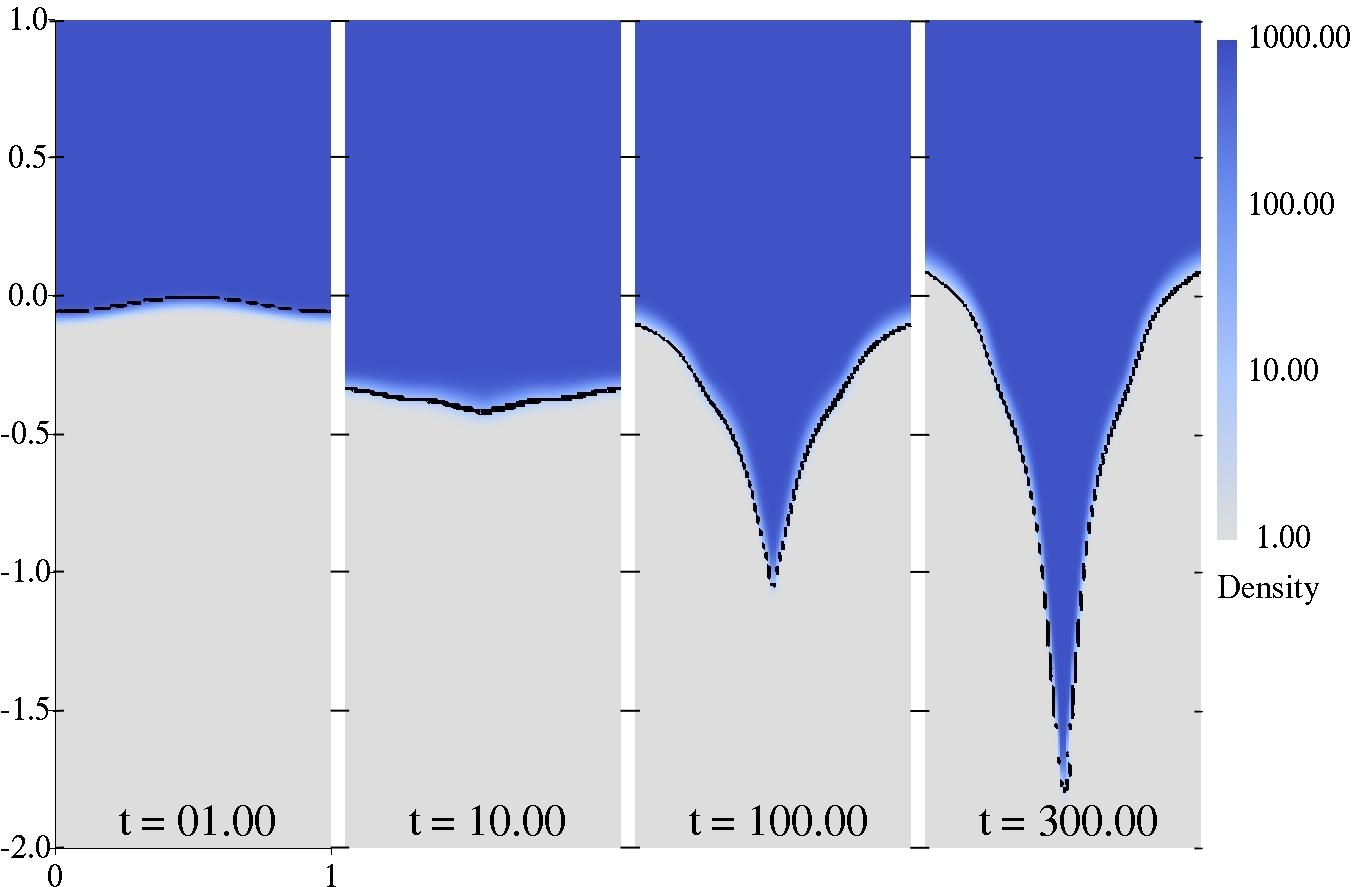
\includegraphics[width=0.9\textwidth]{./figs/lung_figs/snapshots_density_t1}
%\includegraphics[width=0.9\textwidth]{./figs/lung_figs/snapshots_vorticity_t1}
\caption[The evolution of the acoustically perturbed interface]
{Contour plots of density field illustrate the shape and location of
  the interface throughout the evolution of the flow, at
  $t=1, 10, 100, 300$, for the $10$ MPa trapezoidal wave case. Areas
  of high density (i.e., water) are indicated in dark blue. Areas of
  low density (i.e., air) are indicated in white. Constant 0.5 volume
  fraction water contour lines are indicated in black.}
  \label{fig:interface_snapshots}
\end{figure}
%
To illustrate the evolution of the interface, Figure
\ref{fig:interface_snapshots} contains contour plots of the density
during the compression-interface interaction $(t=1)$, shortly after
the wave leaves the interface $(t=10)$, and at late times
$(t=100, 300)$. Contours of 0.5 volume fraction of water are indicated
in black on both plots. The interface perturbation grows from an
initially smooth sinusoid to a sharp point at late times.
%
\begin{figure}[h] 
  \centering
  \includegraphics[width=0.48\textwidth]{./figs/lung_figs/trapz10_intf_schematic}
%  \includegraphics[width=0.48\textwidth]{./figs/lung_figs/trapz10_circ_schematic}
  \includegraphics[width=0.48\textwidth]{./figs/lung_figs/interface_multi-amp_loglog_roe_t1000}
  \caption[The interface perturbation amplitude histories]{The
    interface perturbation amplitude histories (Left) corresponding to
    the $10$ MPa trapezoidal wave case for $t\leq25$, with the times
    at which different stages of the incoming trapezoidal pressure
    wave encounter the interface indicated as $t_{1-4}$. The
    perturbation amplitude histories for the $5$ and $10$ MPa cases
    are plotted for $t\leq1000$ are plotted on logarithmic axes (Right).}
  \label{fig:trapz10_circ_interface}
\end{figure}
%
To more closely exam the interface dynamics associated with the
wave-interface interaction, Figure \ref{fig:trapz10_circ_interface}
shows the early-time histories of the interface amplitude $a(t)$ and
right half-domain circulation $\Gamma$. We have labeled the times at
which different portions of the incoming wave encounter the interface
as $t_{1-4}$, denoted with black $\bs{\times}$s along the curves in
these figures and those hereafter. From $t_1=0^+$ to $t_2$ the
compression wave encounters the interface. We note the average
perturbation amplitude during this period
$\overline{a(t_{1-2})}/a_0\approx0.96$, suggesting that the static
interface assumption made in our vorticity generation order of
magnitude analysis was reasonable. At $t_2\approx1.1$, the pressure
reaches its maximum amplitude, $p_a=10$ MPa, and remains constant
until $t_3$. During this period, the interface amplitude continues to
decrease until $t\approx 5.0$, at which point the perturbation
undergoes a phase inversion and begins to grow. This phase inversion
is also observed for the heavy-light interface Richtmyer-Meshkov
problem. At $t_3\approx8.5$ the expansion wave hits the interface and
the perturbation amplitude continues to grow. At $t_4\approx9.7$ the
acoustic wave has finished traversing the interface, and atmospheric
pressure is resumed. The perturbation amplitude $a(t)$ continues to
increase indefinitely after the wave-interface interaction has
finished.



%
\subsection{Vorticity dynamics}
\begin{figure}[h] 
  \centering
%\includegraphics[width=0.9\textwidth]{./figs/lung_figs/snapshots_vorticity_t1}
  \caption[The evolution of the vorticity] {Contour plots of vorticity
    field throughout the evolution of flow, at
    $t=1, 10, 100, 300$, for the $10$ MPa trapezoidal wave case. Areas
    of positive vorticity are indicated in red. Areas of negative
    vorticity are indicated in blue. Constant 0.5 volume fraction
    water contour lines are indicated in black.}
  \label{fig:interface_snapshots}
\end{figure}





\section{OLD}
%---------------------------------------------------------------------

 vorticity (Bottom) fields at different instances in
the flow's evolution. Areas of high density (i.e., water) are dark
blue and areas of low density (i.e., air) are light-blue. On the
vorticity contours, counterclockwise (positive) vorticity is red, and
clockwise (negative) vorticity is blue. The purpose of the vorticity
plots is only to show the location and direction of vorticity at each
time. For sake of visualization, the range of the vorticity color
scale changes at each time slice because the vorticity spreads over
time. Hence the vorticity magnitudes are not shown here.  

The initially smooth interface perturbation grows from a smooth
sinusoid to a sharp spike at late time.  vorticity is heavily
concentrated in the air. At $t=1$, the compression-interface
interaction has nearly completed and 97\% of the total circulation in
the left or right half domain exists in fluid with volume fraction
$\alpha<0.5$. This is qualitatively consistent with our analysis. As
time progresses, it can be seen that the vorticity disperses
throughout the domain, but remains concentrated around the interface
and the vertical center of the domain.

To more closely exam the interface and circulation dynamics associated
with the compression wave-interface interaction, Figure
\ref{fig:trapz10_circ_interface} shows the early-time histories of the
interface amplitude $a(t)$ and half-domain circulation $\Gamma$. We
have labeled the times at which different portions of the incoming
wave encounter the interface as $t_{1-4}$, denoted with black
$\bs{\times}$s along the curves in these figures and those
hereafter. From $t_1=0^+$ to $t_2$ the compression wave encounters the
interface. During this interaction the perturbation amplitude
decreases, and the right half-domain circulation $\Gamma$ rises
sharply. At $t_2\approx1.1$, the pressure reaches its maximum
amplitude, $p_a=10$ MPa, and remains constant until $t_3$. We note
that at $\overline{a(t_{1-2})}/a_0\approx0.96$, suggesting that the
static interface assumption made in our vorticity generation order of
magnitude analysis was reasonable. The interface amplitude continues
to decrease and the half-domain circulation $\Gamma$ stops its rapid
growth and changes little during this static elevated pressure period,
until the expansion wave hits at $t_3$. At $t\approx 5.0$, the
perturbation undergoes a phase inversion and begins to grow, as is
observed for the heavy-light interface Richtmyer-Meshkov problem. At
$t_3\approx8.5$ the expansion wave first hits the interface. The
perturbation amplitude continues to grow, and $\Gamma$ increases
sharply again. At $t_4\approx9.7$ the acoustic wave has finished
traversing the interface, and atmospheric pressure is resumed. The
perturbation amplitude $a_0$ continues to grow long after the
wave-interface interaction has finished.
%
\begin{figure}[h] 
  \centering
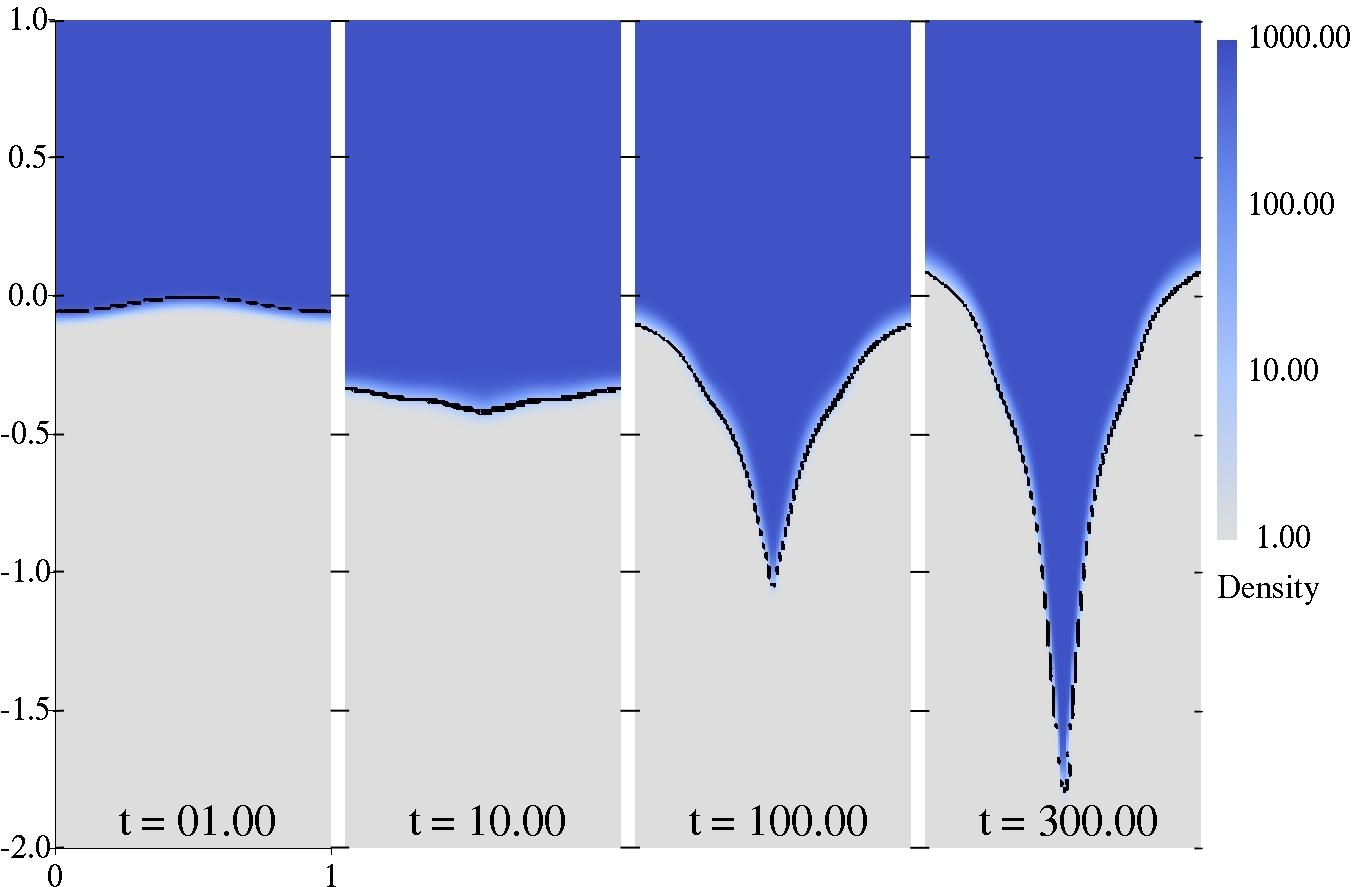
\includegraphics[width=0.9\textwidth]{./figs/lung_figs/snapshots_density_t1}
%\includegraphics[width=0.9\textwidth]{./figs/lung_figs/snapshots_vorticity_t1}
\caption[The evolution of the acoustically perturbed interface and vorticity field]{Surface plots of density (Top) and vorticity (Bottom)
  throughout the evolution of the interface for the $10$ MPa
  trapezoidal wave case. Areas of high density (i.e., water) are
indicated in dark blue. Areas of low density (i.e., air) are indicated
in white.  Positive (counterclockwise) vorticity is indicated in red,
and negative (clockwise) vorticity can be seen in blue.}
  \label{fig:interface_snapshots}
\end{figure}
%
\begin{figure}[h] 
  \centering
  \includegraphics[width=0.48\textwidth]{./figs/lung_figs/trapz10_intf_schematic}
  \includegraphics[width=0.48\textwidth]{./figs/lung_figs/trapz10_circ_schematic}
  \caption[The interface amplitude and circulation histories for the $10$ MPa trapezoidal wave]{The interface amplitude (left) and circulation (right)
    histories corresponding to the $10$ MPa trapezoidal waves are
    shown for $t\leq25$. Indicated times, $t_{1-4}$, are the times at
    which different stages of the incoming trapezoidal pressure wave
    shown in Figure \ref{fig:p0} first encounter the interface.}
  \label{fig:trapz10_circ_interface}
\end{figure}
%
%
\subsubsection{Dependence on acoustic wave amplitude}%
\label{subsubsec:amplitude_dependence}%
To investigate the dependence of the dynamics on the trapezoidal wave
amplitude, we compare results for $p_a=1$, $5$, and $10$ MPa while
keeping the initial lengths of the wave $L$ and the rise and fall
$\Delta L_a$ constant such that $p_a$ scales linearly with the
acoustic pressure gradient. Figure
\ref{fig:trapz_circ_interface_early}, illustrates the interface
amplitude and $p_a$-normalized circulation histories for $t\leq25$,
during and shortly after the wave-interface interaction. Black
$\bs{\times}$s along the curves indicate $t_{1-4}$, described
previously in Subsection \label{subsec:Qualitative}. During the
interaction between the interface and the compression wave, the rate
at which the perturbation amplitude decreases is greater for higher
amplitude waves. The circulation deposited during this period scales
linearly with $p_a$ as is consistent with baroclinically-generated
circulation based on our analysis. For the $10$ MPa wave, the phase of
the interface inverts at, before the expansion hits, causing
circulation deposited by the expansion to have the same sign as that
deposited by the compression. For the $1$ and $5$ MPa waves interface
phase inversion occurs after the expansion and consequently deposits
circulation opposite that of the compression wave.

Figure \ref{fig:trapz_circ_interface_loglog} \hl{(update this figure)}
shows the interface amplitude and circulation histories for $5$ and
$10$ MPa trapezoidal wave cases for $0 \leq t\leq 1000$. The
perturbation amplitude history is plotted on logarithmically-scaled
axes. For both waves, the slope of the perturbation amplitude is
approximately $0.60$ long after the waves have left the
interface. This is slightly higher than the 0.5 slope predicted by
scaling law \eqref{eq:intf_circ_scaling}. The results for the $1$ MPa
trapezoidal wave were not included because interface evolved too
slowly to obtain useful data given the computational resources available.
%
\begin{figure}[h] 
  \centering
  \includegraphics[width=0.48\textwidth]{./figs/lung_figs/interface_multi-amp_norm}
  \includegraphics[width=0.48\textwidth]{./figs/lung_figs/circulation_multi-amp_norm}
  \caption[The interface and circulation dependence on wave amplitude at early time]{The interface amplitude (left) and circulation (right)
    histories corresponding to the $1$(yellow), $5$(orange), and
    $10$(blue) MPa trapezoidal waves are shown for $t\leq 25$. The
    circulation history is normalized by the acoustic amplitude of the
    incoming wave to illustrate that circulation deposition by the
    compression wave scales linearly with $p_a$.}
  \label{fig:trapz_circ_interface_early}
\end{figure}
%
\begin{figure}[h] 
  \centering
  \includegraphics[width=0.48\textwidth]{./figs/lung_figs/interface_multi-amp_loglog_roe_extra}
  \includegraphics[width=0.48\textwidth]{./figs/lung_figs/circulation_multi-amp2_roe}
  \caption[The interface and circulation dependence on wave amplitude
  at long time]{The interface amplitude (left) and circulation (right)
    histories corresponding to the $5$(orange) and $10$(blue) MPa
    trapezoidal waves are shown for $t\leq 500$. To appropriately
    compare late time dynamics, time has been offset in the interface
    amplitude history such that the phase reversal appears to occur
    simultaneously in both simulations. Dashed lines of the same color
    are used to demonstrate the expected slope of pure circulation
    driven interface growth, based on Equation
    \eqref{eq:intf_circ_scaling}. The red dashed line shows the slope we
    appear to be approaching for the $10$ MPa wave case for the end time.}
  \label{fig:trapz_circ_interface_loglog}
\end{figure}
%
\subsubsection{Dependence on the length of the wave}%
To investigate the dependence of the dynamics on the length of the
trapezoidal wave $L$, and comparably the wave-interface interaction
time, we compare results for $p_a=10$ MPa waves of constant rise and
fall length $\Delta L_a$. This effectively changes the time the
interface has to evolve while experiencing the constant elevated
pressure portion of the wave between the compression and expansion.
Figure \ref{fig:trapz_circ_interface_multi-lag} shows the interface
amplitude and circulation histories corresponding to waves with
$L=45\lambda, 35\lambda ,30\lambda ,25\lambda ,15\lambda ,10\lambda$
for $0 \leq t\leq 25$.  For the three longest waves, $L \geq 30\lambda$,
the expansion encounters the interface after the perturbation reverses
phase. In these cases, the expansion deposits additional positive
circulation along the right half of the interface. For the shorter
waves, $L \leq 25\lambda$, the expansion encounters the interface before
the perturbation reverses phase and the net half-domain circulation is
decreased. Comparing cases in which the interface inverts phase before
the expansion occurs the larger $a(t)$ is at the time, the more
circulation is generated. The same is true when comparing cases in
which the phase inversion occurs after the interface inverts phase.
%
\begin{figure}[h] 
  \centering
  \includegraphics[width=0.48\textwidth]{./figs/lung_figs/interface_multi-lag}
  \includegraphics[width=0.48\textwidth]{./figs/lung_figs/circulation_multi-lag_fixed}
  \caption[The interface and circulation dependence on wave
  duration]{The interface amplitude (left) and circulation (right)
    histories for waves of varying total length $L$ and elevated
    static pressure duration between the expansion and compression
    . Here we show results for $L=45\lambda$ (blue), $L=35\lambda$
    (orange), $L=30\lambda$ (yellow), $L=20\lambda$ (purple),
    $L=15\lambda$ (green), $L=10\lambda$ (light blue)}
  \label{fig:trapz_circ_interface_multi-lag}
\end{figure}
%
\subsection{Discussion}
\label{subsec:discussion}
After the passage of the trapezoidal acoustic waves the pressure
returns to the initial, ambient conditions. This implies that the
integral of the pressure gradient $\nabla p$ along the interface, over
all time is zero. Hence we surmise that if the interface remains
unchanged during the interaction with the wave, as it would for a wave
moving with infinite velocity, $\nabla \rho$ would remain constant and
the net baroclinic circulation deposited must be zero. Thus for any
finite duration acoustic wave to deposit net baroclinic circulation
upon an interface, the interface itself must deform during interaction
with the wave. This deformation alters the misalignment of the
pressure and density gradients throughout the passage of the wave such
that vorticity deposited by the compression and expansion waves do not
cancel. Note that this of particular interest for waves in which
the pressure returns to the initial condition after the wave passes,
which is not the case for the traditional shock-accelerated \ac{RMI}
problem.

For the cases varying the length of the wave $L$, we previously noted
that whether the expansion increased or decreased the total
half-domain circulation depended on whether it encountered the
interface before or after the phase change. If indeed circulation is
driving the deformation of the interface, then changes in the waveform
that appear to have very little effect on the interface dynamics
during the wave-interface interaction period, may have far more
significant impacts on the long term dynamics of the interface via
vorticity.

%% Local Variables:
%%% mode: latex
%%% TeX-master: "../main"
%%% End:


\section{Results, analysis, and discussion}%
\label{sec:results}%
% 
In this section we present the results of the numerical experiments
and compare them to our analysis. We focus specifically on the
relationship between circulation and interface dynamics.
% 
%%%%%%%%%%%%%%%%%%%%%%%%%%%%%%%%%%%%%%%%%%%%%%%%%%%%%%%%%%%%%%%%%% 
%%%%%%%%%%%%%%%%%%%%%%%%%%%%%%%%%%%%%%%%%%%%%%%%%%%%%%%%%%%%%%%%%% 
%%%%%%%%%%%%%%%%%%%%%%%%%%%%%%%%%%%%%%%%%%%%%%%%%%%%%%%%%%%%%%%%%% 
%%%%%%%%%%%%%%%%%%%%%%%%%%%%%%%%%%%%%%%%%%%%%%%%%%%%%%%%%%%%%%%%%% 
% 
\subsection{Qualitative observations of the interface response to the trapezoidal wave}
\label{subsec:Qualitative}
To provide a qualitative understanding of the physics underlying the
wave-interface interaction, we consider a base reference case in which
a $p_a=10$ MPa trapezoidal wave, of length $L=45\ell$, (See Figure
\ref{fig:p0}) impinges from water onto the water-air interface. Nearly
all of the acoustic energy is reflected back into the water as a
tension wave due to the sharp decrease in acoustic impedance across
the interface. The transmitted compression wave is weakly focused due
to the sound speed mismatch across the curved interface
perturbation. The reflected and transmitted waves dissipate at the
inflow and outflow boundaries.
% 
\begin{figure}[h] 
  \centering
  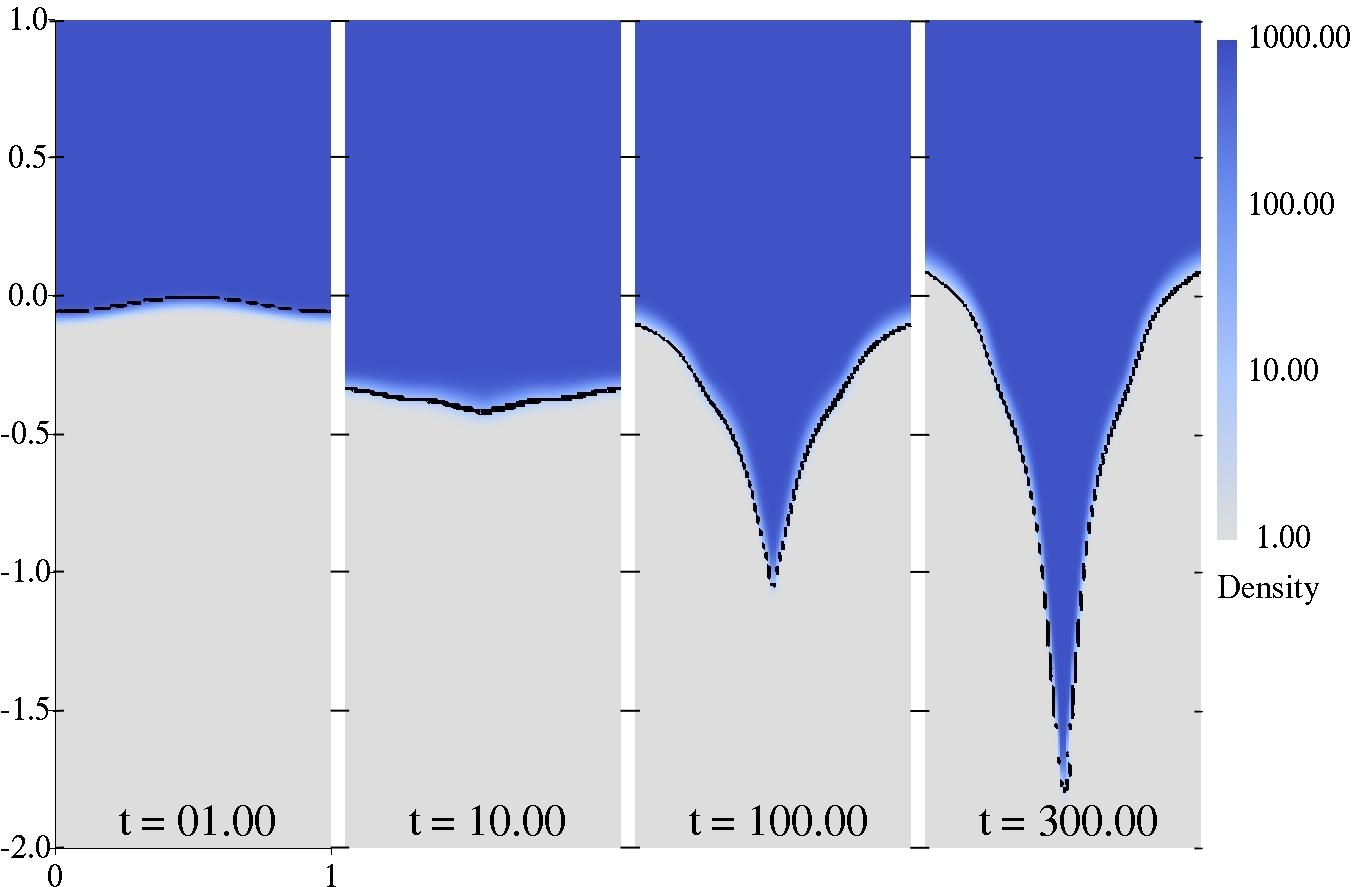
\includegraphics[width=0.9\textwidth]{./figs/lung_figs/snapshots_density_t1}
  \caption[The evolution of the acoustically perturbed interface]
  {Contour plots of density field illustrate the shape and location of
    the interface throughout the evolution of the flow, at
    $t=1, 10, 100, 300$, for the $10$ MPa trapezoidal wave case. Areas
    of high density (i.e., water) are indicated in dark blue. Areas of
    low density (i.e., air) are indicated in light blue. Constant volume
    fraction of water $\alpha = 0.5$ contour lines are indicated in black.}
  \label{fig:interface_snapshots}
\end{figure}
% 
Figure \ref{fig:interface_snapshots} illustrates the evolution of the interface. Contour plots of the density
during the compression-interface interaction $(t=1)$, shortly after
the wave leaves the interface $(t=10)$, and at late times
$(t=100, 300)$ are shown. Note that all times and lengths presented are
dimensionless such that $t = \text{Time}/\left(\ell/c_{air}\right)$ and $x$,
$y$ are nondimensionalized by $\ell$. High-density regions (i.e.,
water) are indicated in dark blue. Low-density regions (i.e., air) are
indicated in light-blue. Isocontours of volume fraction of water
$\alpha=0.5$ are indicated in black. The interface
perturbation grows from an initially smooth sinusoid to a sharp point
at late times, long after all waves have left the domain.
% 
\begin{figure}[h] 
  \centering
  \begin{subfigure}[b]{0.45\textwidth}
    \centering
    \includegraphics[width=\textwidth]{./figs/lung_figs/trapz10_intf_schematic.pdf}
    \caption{\label{fig:trapz10_interface25} $0\leq t \leq 25$.}
  \end{subfigure}
  ~
  \begin{subfigure}[b]{0.45\textwidth}
    \centering
    \includegraphics[width=\textwidth]{./figs/lung_figs/trapz10_intf_t1000.pdf}%
    \caption{\label{fig:trapz10_interface1000} $0\leq t \leq 1000$.}
  \end{subfigure}
  \caption[The interface perturbation amplitude history for 10 MPa
  trapezoidal wave]{The interface perturbation amplitude $a(t)$ for
    the $10$ MPa trapezoidal wave case for $t\leq25$ in Figure \protect\subref{fig:trapz10_interface25} and for
    $t\leq1000$ in Figure \protect\subref{fig:trapz10_interface1000}. The times at which different stages of the
    incoming trapezoidal pressure wave encounter the interface are
    indicated as in Figure \protect\subref{fig:trapz10_interface25} as $t_{1-4}$.}
  \label{fig:trapz10_interface}
\end{figure}\par
% 
To more closely exam the interface dynamics in the period surrounding
the wave-interface interaction, Figure \ref{fig:trapz10_interface25}
shows the interface perturbation amplitude nondimensionalized by its
initial value $a(t)/a_0$ for $t\leq25$, the period during and shortly
after the wave-interface interaction. We have labeled the times at
which different portions of the incoming wave encounter the interface
as $t_{1-4}$, denoted with black $\bs{\boldsymbol{\times}}$s along the
curves. From $t_1=0^+$ to $t_2\approx1.1$ the compression wave
encounters the interface. At $t_2$, the incoming pressure reaches its
maximum amplitude, $p_a=10$ MPa, and remains constant until
$t_3\approx8.5$. During this period, the interface amplitude continues
to decrease until the perturbation undergoes a
phase inversion at $t\approx 5.0$ and begins to grow. This phase inversion is similar to
that observed for the heavy-light interface Richtmyer-Meshkov
problem. At $t_3$ the pressure expansion hits the interface and the
perturbation amplitude continues to grow. At $t_4\approx9.7$ the
acoustic wave has finished traversing the interface, and the interface
pressure is nominally atmospheric. Figure
\ref{fig:trapz10_interface1000} shows $a(t)/a_0$ for $t\leq1000$. The
interface amplitude continues to grow indefinitely, long after all
acoustic waves have left the domain and the pressure field has
returned to atmospheric. In the absence of viscosity or other loss
mechanisms, this is expected. At late times, vorticity remains to
drive the deformation of the interface.
% 
%%%%%%%%%%%%%%%%%%%%%%%%%%%%%%%%%%%%%%%%%%%%%%%%%%%%%%%%%%%%%%%%%% 
%%%%%%%%%%%%%%%%%%%%%%%%%%%%%%%%%%%%%%%%%%%%%%%%%%%%%%%%%%%%%%%%%% 
%%%%%%%%%%%%%%%%%%%%%%%%%%%%%%%%%%%%%%%%%%%%%%%%%%%%%%%%%%%%%%%%%% 
%%%%%%%%%%%%%%%%%%%%%%%%%%%%%%%%%%%%%%%%%%%%%%%%%%%%%%%%%%%%%%%%%% 
% 
\subsection{Vorticity and circulation dynamics}
\begin{figure}[h] 
  \centering
  %\includegraphics[width=0.9\textwidth]{./figs/lung_figs/snapshots_vorticity_t1}
  \includegraphics[width=0.98\textwidth]{./figs/lung_figs/vorticity_snapshot_mat}
  \caption[The evolution of the vorticity] {Contour plots of vorticity
    field throughout the evolution of flow, at $t=1, 10, 100, 300$,
    for the $10$ MPa trapezoidal wave case. Areas of positive
    vorticity are indicated in red. Areas of negative vorticity are
    indicated in blue. Constant volume fraction of water $\alpha=0.5$
    contour lines are indicated in black. As this plot is designed
    only to illustrate the location of vorticity, the color scale
    changes at each time and its values are not indicated here.}
  \label{fig:vorticity_snapshots}
\end{figure}
% 
To explain the continued growth of the interface at late times, we
look to vorticity. Figure \ref{fig:vorticity_snapshots} shows
contour plots of the vorticity field at $t=1, 10, 100, 300$, for the
$10$ MPa trapezoidal wave case. Areas of positive (counter-clockwise)
vorticity are indicated in red. Areas of negative (clockwise)
vorticity are indicated in blue. As the purpose of this plot is to
visualize the location of vorticity, the color scale changes at each
time step and is not indicated on this plot. The position of the
interface is indicated by black contour lines of constant volume
fraction of water $\alpha=0.5$. At $t=1$, near the end of the
compression-interface interaction, the bulk of the vorticity is in
air-dominated fluid. As the perturbation grows, vorticity bleeds
across the interface. Vorticity remains concentrated around the middle
of the interface and in its wake.

To better understand the vorticity dynamics we consider the vorticity
generation equation for a 2D, inviscid fluid system,
\begin{align} \label{eq:vorticity_euler}
  \frac{\partial \boldsymbol{\omega}}{\partial t}+\left(\boldsymbol{u}\cdot\nabla\right)\boldsymbol{\omega} =% 
  - \boldsymbol{\omega}\left(\nabla\cdot\boldsymbol{u}\right) + \frac{\nabla\rho\times\nabla p}{\rho^2}.%
\end{align}

Each term in equation \eqref{eq:vorticity_euler} represents a
different physical mechanism by which the vorticity
$\boldsymbol{\omega}$ is changing. Terms on the left-hand side
represent changes in the existing vorticity field and terms on the
right represent vorticity sources and sinks. On the left, the first
term represents the total change of vorticity at a location in the
flow field with respect to time and the second term represents the
advection of vorticity. On the right, the first term describes changes
in vorticity due to compressibility, and the second term is the
baroclinic term which describes vorticity generated by the
misalignment of the pressure and density gradients. We
seek to understand the relative importance of these mechanisms on the
dynamics of the acoustically accelerated interface.
% 
%%%%%%%%%%%%%%%%%%%%%%%%%%%%%%%%%%%%%%%%%%%%%%%%%%%%%%%%%%%%%%%%%% 
%%%%%%%%%%%%%%%%%%%%%%%%%%%%%%%%%%%%%%%%%%%%%%%%%%%%%%%%%%%%%%%%%% 
%%%%%%%%%%%%%%%%%%%%%%%%%%%%%%%%%%%%%%%%%%%%%%%%%%%%%%%%%%%%%%%%%% 
%%%%%%%%%%%%%%%%%%%%%%%%%%%%%%%%%%%%%%%%%%%%%%%%%%%%%%%%%%%%%%%%%% 
% 
\subsubsection{Order of magnitude analysis of vorticity generation mechanisms}
\label{subsubsec:oom_analysis}
To quantifiably compare the various mechanisms by which vorticity
changes within the flow we perform an order of magnitude analysis on
each term of the vorticity generation equation
\eqref{eq:vorticity_euler}.

To determine the appropriate time and location for the analysis, we
recognize that the flow is initially free of vorticity and any
vorticity generated must be a result of acoustic energy being
converted to kinetic energy in the flow. The only mechanism for
this to occur in an inviscid fluid without pre-existing vorticity is
baroclinicity. Thus we require misaligned density and pressure
gradients. The greatest density gradients in the flow occur across the
interface. The strongest pressure gradients occur in the acoustic
wave. Hence we choose to perform our analysis at the water-air
interface during the wave-interface interaction.

For simplicity, we consider specifically the time in which the
compression interacts with the interface. This interaction occurs
quickly, over approximately $\Delta t_a\approx5\ell/c_{w}$. As such we
treat the interface as static and undeformed during this
interaction. Based on the results presented in Figure
\ref{fig:trapz10_interface}, the average perturbation amplitude during
this period is $<a(t_{1-2})>\approx0.96\ a_0$, suggesting that this
assumption is reasonable for order of magnitude analysis.

To evaluate the order of magnitude of the individual terms of the
vorticity generation equation \eqref{eq:vorticity_euler}, we treat
gradient, curl, and divergence of any arbitrary quantity $f$ such that
$\abs{\nabla} f= \orderof{\left|\Delta f\right|/\Delta L}$,
$\nabla\cdot f=\orderof{\left|\Delta f\right|/\Delta L}$, and
$\nabla\times f=\orderof{\left|\Delta f\right|/\Delta L}$. Here
$\Delta f$ is a change in $f$ over a characteristic length scale
$\Delta L$. As the only motion in the flow is generated by the
acoustic wave, we consider acoustic pressure, velocity, and density
perturbations such that $\Delta p=\Delta p_a$,
$\Delta \boldsymbol{u}=\Delta \boldsymbol{u}_a$, and
$\Delta \rho=\Delta \rho_a$. The subscript $_a$ denotes acoustic
quantities. We use acoustic relations to relate these quantities
\citep{Anderson1990},
\begin{align}%
  \label{eq:acoustic_relations}%
  \Delta p_a=\pm\Delta u_a \rho c=c^2\Delta \rho_a.%
\end{align}

To assess the baroclinic contribution to vorticity, we write the cross
product of the density and pressure gradients as
$\abs{\nabla \rho} \abs{\nabla p} \sin{\left(\theta\right)}$. Here
$\theta$ is the angle between the acoustic pressure gradient, treated
as being in the $\plus y$-direction, and the direction of the density
gradient which we treat as the outward normal direction to the
interface. For $a_0/\ell<<1$, we can approximate
$\sin{\left(\theta\right)}\approx\theta$ at the interface. The density
gradient due to the water-air interface is far greater than that due
to the acoustic wave. As such we use the change in density across the
interface $\Delta \rho_I$ and associated length scale $\Delta L_I$ to
write the density gradient. The pressure change is a result of the
acoustic wave, and as such we use the acoustic pressure change
$\Delta p_a$ and associated length scale $\Delta L_a$ to express the
pressure gradient. And thus we write the order of magnitude of the
baroclinic vorticity generation term at the interface,
\begin{align}
  \label{eq:baroclinic_vorticity}%
  \norm{\frac{\nabla\rho\times\nabla p}{\rho^2}} =%
  \orderof{\frac{\abs{\Delta \rho_I}}{\abs{\Delta L_I}}\frac{\abs{\Delta p_a}}{\abs{\Delta L_a}}\frac{1}{\abs{\rho}^2}\abs{\theta}}.%
\end{align}

In the evaluation of the compressible and advective terms we consider
two possible evaluations of the vorticity $\omega$ as either the curl
of the acoustic velocity field
$\boldsymbol{\omega}=\nabla\times\boldsymbol{u}$ or the integral of
the baroclinic vorticity generation term from
\eqref{eq:baroclinic_vorticity}, treated as constant, over the
characteristic time of the pressure rise
$\Delta t_a\approx\Delta L_a/c_w$. Evaluating the vorticity using both
of these expressions and the values presented later in this section
reveals that the baroclinic expression of the vorticity is dominant
for the regimes of interest to this study and is thus what we will use
this treatment in our further analysis. Hence the approximate order of magnitude of the compressible and
advective vorticity generation is written as
\begin{align}
  \label{eq:compressible_advective_vorticity}%
  \norm{-\boldsymbol{\omega}\left(\nabla\cdot\boldsymbol{u}\right)}\sim \norm{\left(\boldsymbol{u}\cdot\nabla\right)\boldsymbol{\omega}} = %
  \orderof{%
  \frac{\abs{\Delta u_a}}{\abs{\Delta L_a}} \frac{\abs{\Delta \rho_I}}{\abs{\Delta L_I}}%
  \frac{\abs{\Delta p_a}}{\abs{\Delta L_a}} \frac{1}{\abs{\rho}^2}\abs{\theta}\frac{\abs{c}}{\abs{\Delta L_a}}%
  }.%
\end{align}

Now, to compare the relative importance of the baroclinic and
compressible (or advective) contributions to vorticity we will look at
the ratio of the two vorticity generation approximations. We divide
equation \eqref{eq:baroclinic_vorticity} by equation
\eqref{eq:compressible_advective_vorticity} using
\eqref{eq:acoustic_relations} to express acoustic quantities in terms
of the acoustic perturbation quantities $\Delta \rho_a,\,\Delta u_a$ and simplify,
\begin{align} \label{eq:vorticity_comparison}
  \frac{\norm{\frac{\nabla\rho\times\nabla
  p}{\rho^2}}}{\norm{-\boldsymbol{\omega}\left(\nabla\cdot\boldsymbol{u}\right)}}
  \sim
  \frac{\norm{\frac{\nabla\rho\times\nabla
  p}{\rho^2}}}{\norm{\left(\boldsymbol{u}\cdot\nabla\right)\boldsymbol{\omega}}}
  = \orderof{\frac{\abs{c}}{\abs{\Delta u_a}}} = \orderof{\frac{\abs{\rho}}{\abs{\Delta \rho_a}}}%
\end{align}

To evaluate the above expressions for comparison with our
computational results, we consider our base trapezoidal wave case
where $p_a = \Delta p_a = 10$ MPa. The length scale associated with
the acoustic wave is the initial length of the pressure rise
$\Delta L_a=5\ell$. The initial interface length scale
$\Delta L_I$, defined as the thickness of the thickness of the mixed
layer from $\alpha=0.05$ to $0.95$ volume fraction of water is estimated
as $\Delta L_I \approx 0.05\ell$. We approximate the order of theta
based on its average value along a half-wavelength of the interface
for $a_0=0.03\ell$ such that
$<\abs{\theta}>\approx0.12$. Evaluating expression
\eqref{eq:vorticity_comparison} we to find that
$\abs{c}/\abs{\Delta u_a}$=247 and thus expect that the relative
contribution of baroclinic to compressible/advective vorticity
generation is approximately of order $\orderof{10^2}$ at
$t=\Delta t_a=1.05$.

To compare our computational results to the analysis we consider the
integral of the vorticity and vorticity generation terms over the
right-half domain,
\begin{align}
  \Gamma = \int_{A_{RH}} \omega \,dA_{RH},
\end{align}
where
$\int_{A_{RH}} dA_{RH} =
\int_{-\infty}^{+\infty}\int_{\ell/2}^{\ell} \,dy\, dx$. Note
that the right-half domain is considered because the total circulation
over the whole domain is $0$ due to symmetry. Circulation is chosen as
the quantity of comparison as it is a global quantity, which better
captures the overall vorticity dynamics than the vorticity at any
single point. As a single quantity rather than a field, it is also
simpler to compare the computational and analytical results. The
relative order of magnitude relationships obtained in
\eqref{eq:vorticity_comparison} are spatially independent and expected
to hold when integrated over the right-half domain. Accordingly we
evaluate the vorticity generation terms from our computational results
integrated over the right-half domain. At $t=1.0$ we find that %
$$ \int_{A_{RH}} \left[\frac{\nabla\rho\times\nabla p}{\rho^2}\right] / \left[\left(\boldsymbol{u}\cdot\nabla\right)\boldsymbol{\omega}\right]\,\,dA_{RH}\approx 285=\orderof{10^2}$$
and
$$ \int_{A_{RH}} \left[\frac{\nabla\rho\times\nabla p}{\rho^2}\right] / \left[-\boldsymbol{\omega}\left(\nabla\cdot\boldsymbol{u}\right)\right]\,\,dA_{RH} \approx 145=\orderof{10^2}.$$
%
hence the computational results and analysis are in agreement and suggest
that the vorticity is nearly entirely baroclinic.
% 

\subsubsection{Circulation deposition}
Having established that the circulation is a primarily result of
baroclinic vorticity, we now look to understand the circulation
deposition associated with the wave-interface interaction period.
%
\begin{figure}
  \centering
  \begin{subfigure}[b]{0.48\textwidth}
    \centering
    \includegraphics[width=\textwidth]{./figs/lung_figs/trapz10_circ_schematic.pdf}
    \caption{\label{fig:trapz10_circ_schematic_t25} $0\leq t \leq 25$ }
  \end{subfigure}
  ~
  \begin{subfigure}[b]{0.48\textwidth}
    \centering
    \includegraphics[width=\textwidth]{./figs/lung_figs/Gamma_t1000_28-Oct-2016.pdf}
    \caption{\label{fig:trapz10_circ_schematic_t1000} $0\leq t \leq 1000$}
  \end{subfigure}
  %
  \caption[Circulation deposition by the 10 MPa trapezoidal wave] {The
    circulation history for the right-half domain is shown for the 10
    MPa trapezoidal wave case for $t\leq25$ in Figure
    \protect\subref{fig:trapz10_circ_schematic_t25} and for
    $t\leq1000$ in Figure
    \protect\subref{fig:trapz10_circ_schematic_t1000}. The times at
    which different stages of the incoming trapezoidal pressure wave
    encounter the interface are indicated in Figure
    \protect\subref{fig:trapz10_circ_schematic_t25} as $t_{1-4}$.}
  \label{fig:trapz10_circ_schematic}
\end{figure}

Figure \ref{fig:trapz10_circ_schematic}, shows circulation history of
the right-half domain for the $10$ MPa wave case for $t\leq25$, during
and shortly after the wave-interface interaction, and for the duration
of the simulation, $t\leq1000$. The points at which the different
components of the wave encounter the interface are indicate as
$t_{1-4}$, as described in section \ref{subsec:Qualitative}.

From $t_1=0^+$ to $t_2$ the compression wave encounters the interface
and $\Gamma$ increases. From $t_2\approx1.1$ to $t_3\approx8.5$ the
pressure gradient at the interface is small and $\Gamma$ changes
little. From Figure \ref{fig:trapz10_interface}, the perturbation
undergoes a phase inversion at $t\approx 5.0$, and hence the density
gradient along the interface reverses direction around this point in
time. At $t_3\approx8.5$ the expansion wave first hits the
interface. The pressure and density gradients at the interface have
both reversed sign since the initial compression wave-interface
interaction and $\Gamma$ increases sharply again. At
$t_4\approx9.7$ the acoustic wave has finished traversing the
interface and ceases depositing vorticity around the interface.

\subsubsection{Circulation-driven, late-time growth of the interface}
\begin{figure}
  \centering
  \begin{subfigure}[t]{0.45\textwidth}
    \centering
    \includegraphics[height=0.8\textwidth]{./figs/lung_figs/a0_t1000_23-Dec-2016}
    \caption{\label{fig:trapz_interface_t1000} Constant scaling: $a(t)/a_0$}
  \end{subfigure}
  ~
  \begin{subfigure}[t]{0.45\textwidth}
    \centering
    \includegraphics[height=0.8\textwidth]{./figs/lung_figs/intf_amp_t1000_23-Dec-2016}
    \caption{\label{fig:trapz_interface_t1000_scaled} Vortex strength scaling: $a(t)/\left(\frac{\Gamma_0}{s_0}\frac{\ell}{c}\right)$}
  \end{subfigure}
  %
  \caption[The interface amplitude at long time]{The interface
    amplitude histories corresponding to the $5$ (blue), $7.5$ (red),
    $10$ (green), and $12.5$ (Purple) MPa trapezoidal waves are shown
    for $t\leq 1000$. \subref{fig:trapz_interface_t1000} shows the
    interface amplitudes $a(t)$ scaled by a constant
    $a_0=0.03\ell$. \protect\subref{fig:trapz_interface_t1000_scaled}
    shows the interface amplitude scaled by $\Gamma_0/s_0$, the
    circulation per unit arc length of the interface at the time at
    when vorticity becomes the dominant mechanism driving the motion
    of the interface. This scaled amplitude is nondimensionalized by
    constants $\ell$ and $c_{air}$. The time for each curve has been
    synced to align the phase inversion of the interface. The black
    dashed line above the curves at late times corresponds to power
    law growth with $t^{3/5}$.}
  \label{fig:trapz_interface_loglog}
\end{figure}

In consideration of the late time growth, Figure
\ref{fig:trapz_interface_loglog} shows the interface amplitude
$a(t)/a_0$ as a function of time for $5$ (blue), $7.5$ (red), $10$
(green), and $12.5$ (Purple) MPa trapezoidal waves for
$0 \leq t\leq 1000$. From the figure, we observe that at late times
the growth of the interface appears to grow at a fairly constant rate
and appears asymptotic in nature. To explain this, we consider the
case circulation-driven growth of the interface. For this regime, we
expect the perturbation amplitude to depend on the total circulation
$\Gamma$, time $t$, and the material and geometric properties of the
flow setup such as the arc length interface $s$, the transverse
distance between peaks of the interface $\ell$, and the speed of sound
$c$, such that

\begin{align}
  \label{eq:dimensional_amplitude}
  a(t)=f\left(\Gamma, s, \ell, c, t\right).
\end{align}

We hypothesize that growth will specifically depend on concentration
of circulation along the interface, such that we consider the
circulation per unit arc length or the linear circulation density
$\Gamma/s$ as a single variable. Furthermore, we choose to evaluate
these quantities at the specific moment when our assumption of a
circulation-driven interface becomes valid. Thus we evaluate
$\Gamma/s$ at the instant in time in which the circulation becomes the
dominant mechanism driving the motion of the interface. Initially
after the wave encounters the interface, there is little vorticity and
entire interface is accelerated downward by the increased acoustic
pressure in the water. As the acoustic pressure drops and vorticity
around the interface remains or increases, at some time $t_\Gamma$,
the circulation begins to dominate the motion of the interface. This
is observed to occur when the peaks and troughs of the interface,
driven by opposing vortex pairs, begin to move in opposite
directions. The linear circulation density at $t_\Gamma$ will be
denoted as $\Gamma_0/s_0$. For the cases shown, the positive acoustic
pressure in the water drives the entire interface downward, in the
$-y$-direction, until at $t_\Gamma\approx9.4$ the vorticity overcomes
the decreasing acoustic pressure in the water and the $y-$velocity of
the bubble or interface peak becomes positive.

Thus by treating $\Gamma$ and $s$ as a single variable $\Gamma_0/s_0$
and nondimensionalizing Equation \eqref{eq:dimensional_amplitude} by
constants values $\ell$ and $c=c_{air}$ we arrive at a dimensionless
expression of the perturbation amplitude as a function of time,
%
\begin{align}
  \label{eq:dimensionless_groups}
  \frac{a(t)}{\ell}=F\left(\frac{\Gamma_0}{s_0 c}, \frac{t c}{\ell} \right).
\end{align}
%
Furthermore, we expect $a(t)$ to scale linearly with $\Gamma_0/s_0$
such that we write
%
\begin{align}
  \label{eq:dimensionless_relationship}
  a(t)=\frac{\Gamma_0}{s_0}F\left(\frac{t c}{\ell} \right).
\end{align}
%
To test this hypothesized relationship
\eqref{eq:dimensionless_relationship}, we scale the amplitude by the
appropriate circulation density, and plot
$a(t)/\left(\frac{\Gamma_0}{s_0}\frac{c}{l}\right)$ in Figure
\ref{fig:trapz_interface_t1000_scaled}, thereby collapsing the
interface amplitude curves along the vertical direction. To collapse
the data along the horizontal direction, time is shifted to sync the
interface phase inversion for each case. The apparently asymptotic
growth observed suggests power law growth in time, and plotting on a
log-log scale reveals that the perturbation amplitude grows
approximately as $t^{3/5}$, which is indicated by the black dashed
line. Calculated growth goes as $t^n$ where
$n=0.61 (5 \text{MPa}), 0.59 (7.5 \text{MPa}), 0.61 (10 \text{MPa})$
and $0.66 (12.5 \text{MPa})$. To explain the discrepancy, in the $12.5$
MPa case, Figure shows the circulation as a function of time for each
case. Note that for the $5-10$ MPa cases, the circulation is
relatively constant after the passage of the wave. For the $12.5$ MPa
case, there is sufficient baroclinic vorticity deposited by the wave
to generate additional vorticity at late times.
%
\begin{figure}
  \centering
  \includegraphics[height=0.45\textwidth]{./figs/lung_figs/Circulation_t1000_23-Dec-2016}
  \caption[The circulation long time]{The circulation histories
    $\Gamma(t)$ corresponding to the $5$ (blue), $7.5$ (red), $10$
    (green), and $12.5$ (Purple) MPa trapezoidal waves are shown for
    $t\leq 1000$. }
  \label{fig:trapz_circ_t1000}
\end{figure}
%
To quantify the deformation of the interface in cases where the
circulation experiences appreciable change, such as those observed in
the 12.5 MPa case, we have to consider the relationship between the
circulation and the arc-length of the interface. Much like the
perturbation amplitude $a(t)$, we expect change in the arc length of
the interface $s$ to depend on the circulation $\Gamma$ and time
$t$.
%
\begin{align}
  \label{eq:s_dependencies}%
  s(t) = g\left(\Gamma(t), t \right).%
\end{align}%
%
However, the circulation itself initially depends on the geometric and
material properties of the interface during the interaction and then
continues to evolve in time such that for constant wave shape we
expect
%
\begin{align}%
  \label{eq:gamma_dependencies}%
  \Gamma(t) = h\left(p_a, \rho, c, \ell, t\right).%
\end{align}%
%
Previously, we treated the circulation density as a single quantity to
as the two are intrinsically linked. Here, we will do this again, but
in consideration of the interface deformation we now consider the
inverse quantity, the interface arc length per unit circulation
$s(t)/\Gamma(t)$. Thus by appropriately combining equations
\eqref{eq:s_dependencies} and \eqref{eq:gamma_dependencies} we find
that
%
\begin{align}%
  \label{eq:scp_dependencies}%
  \frac{s(t)}{\Gamma(t)} = \psi\left(p_a,\rho, c, \ell, t,\right).
\end{align}%
%
Nondimensionalizing by $\rho$ $c$ and $\ell$,
%
\begin{align}%
  \label{eq:scp_dimensionless}%
  \frac{s(t)}{\Gamma(t)} c = \Psi\left(\frac{p_a}{\rho c^2},\frac{c}{\ell}t,\right).%
\end{align}%
%
Experimental results are used to determine this functional
relationship more precisely. Figure \ref{fig:trapz_scp_t1000} shows
the arc length of the interface per unit circulation as a function of
time, scaled by the input pressure amplitude $p_a$ and
nondimensionalized by the density and sound speed of air for $5$
(blue), $7.5$ (red), $10$ (green), and $12.5$ (Purple) MPa trapezoidal
waves. Time is shifted such that interface phase inversion is synced
for each case. For the $7.5$, $10$, and $12.5$ MPa waves the interface
arc length per unit circulation grows as $t^{1/2}$ and these curves
collapse upon one another when scaled by the input pressure
amplitude. 

Based on the described results and Equation \eqref{eq:scp_dimensionless} we find that 
\begin{align}
  \label{eq:scp_relationship}
  \frac{s(t)}{\Gamma(t)} = \mathcal{C}\frac{\rho}{p_a}\left(\frac{c^3t}{\ell}\right)^{1/2}.
\end{align}
The result from the $5$ MPa case differs from the others in
two ways. First, the value of $s(t)/\Gamma(t)$ does not collapse with
the other curves at late time and second, this quantity does not
achieve $t^{1/2}$ by the end of the simulation. There are a few things
that could be contributing to this. For this case in particular, the
expansion wave encounters the interface nominally simultaneously with
the phase-inversion. This is when the interface is at its flattest,
and as a result, there is not much circulation contributed by the
expansion, because the pressure and density gradients are
aligned. However, the expansion does serve to accelerate the interface
and stretch the perturbations in the interface length, such that it
drives the circulation density to decrease, creating a slightly
different initial condition at the start of the circulation-driven
regime than is observed in the other cases. Furthermore, unlike the
other cases, the circulation density in the $5$ MPa case has not
reached asymptotic behavior at the end of the simulation, so it is not
surprising that the $t^{1/2}$ growth has not yet been
achieved. Running the simulation to asymptotic behavior was
prohibitively computationally expensive in this case.

\begin{figure}
  \centering
  \includegraphics[height=0.45\textwidth]{./figs/lung_figs/scp_t1000_23-Dec-2016}
  \caption[The interface arc length at long times]{The arc length of
    the interface per unit circulation or inverse circulation density
    $s(t)/\Gamma(t)$ is plotted as function of time for the $5$
    (blue), $7.5$ (red), $10$ (green), and $12.5$ (Purple) MPa
    trapezoidal waves for $10\geq t\leq 1000$. The data is scaled by
    the input pressure $p_a$ and non-dimensionalized using constants
    $\ell$ and $c_{air}$. Time is synced such that the interface
    phase-inversion occurs simultaneously in each case.}
  \label{fig:trapz_scp_t1000}
\end{figure}
% 
\subsubsection{Dependence on transient wave-interface interactions}%
\begin{figure}
  \centering
  \includegraphics[width=0.48\textwidth]{./figs/lung_figs/interface_multi-lag}
  \includegraphics[width=0.48\textwidth]{./figs/lung_figs/circulation_multi-lag_fixed}
  \caption[The interface and circulation dependence on wave
  duration]{The interface amplitude (left) and circulation (right)
    histories for waves of varying total length $L$ and elevated
    static pressure duration between the expansion and compression
    . Here we show results for $L=45\ell$ (blue), $L=35\ell$ (orange),
    $L=30\ell$ (yellow), $L=20\ell$ (purple), $L=15\ell$ (green),
    $L=10\ell$ (light blue)}
  \label{fig:trapz_circ_interface_multi-lag}
\end{figure}
Lastly, we investigate the dependence of the interface and circulation
dynamics on the evolution of the interface that occurs during the
wave-interface interaction. To study this, we vary the duration of the
static elevated pressure that the interface experiences between the
compression and expansion of the trapezoidal wave. For our setup, this
is equivalent to changing initial length of the trapezoidal wave $L$,
while keeping constant the wave amplitude $p_a=10$ MPa and the lengths
of the pressure rise and fall $\Delta L_a$. 

Figure \ref{fig:trapz_circ_interface_multi-lag} shows the interface
amplitude and circulation histories corresponding to waves with
$L=45\ell, 35\ell ,30\ell ,25\ell ,15\ell ,10\ell$ for $t\leq 25$.
For the two longest waves, $L=35\ell, 45\ell$, the expansion
encounters the interface appreciably after the perturbation reverses
phase. In these cases, the expansion deposits additional positive
circulation along the right half of the interface. For the shorter
waves, $L \leq 25\ell$, the expansion encounters the interface before
the perturbation reverses phase and the net half-domain circulation is
decreased. For the $L=30\ell$ case, the expansion hits the interface
very shortly after the interface phase-reversal, when the interface is
nearly flat. As a result of this, the pressure gradient and density
gradient are closely aligned and very little circulation is generated
by the expansion wave.

Among cases for which the interface inverts phase before encountering
the expansion, the larger the perturbation amplitude $a(t)$ at the
time of the expansion, the greater the circulation generated. This is
a result of the consequence misalignment in density and pressure
gradients. The same is true when comparing cases for which the
interface inverts phase before encountering the expansion. After the
passage of the acoustic wave and all reflections the pressure returns
to the initial, atmospheric conditions. This implies that the integral
of the pressure gradient $\nabla p$ along the interface, over all time
is zero. If the interface remains unchanged during the interaction
with the wave, as it would for a wave moving with infinite velocity,
$\nabla \rho$ would remain constant and the net baroclinic circulation
deposited must be zero. Thus for any finite duration acoustic wave to
deposit net baroclinic circulation upon an interface, the interface
itself must deform during interaction with the wave. This deformation
alters the misalignment of the pressure and density gradients
throughout the passage of the wave such that vorticity deposited by
the compression and expansion waves do not cancel. This of particular
interest for waves in which the pressure returns to the initial
condition after the wave passes, which is not the case for the
traditional shock-accelerated \ac{RMI} problem.

%============================== Conclusions ================
\section{Summary and Conclusions}
\label{sec:conclusions}
This paper demonstrates that acoustic waves may trigger significant
deformation of perturbed liquid-gas interfaces over long periods of
time. The driving mechanism behind this deformation is baroclinic
vorticity, which occurs as a result of misalignment between the
pressure gradient of the acoustic wave and density gradient of the
perturbed interface. To demonstrate this we simulate trapezoidal
acoustic waves of MPa-order amplitude impinging from water onto a
perturbed air interface air.

The work presented here supports the following three conclusions: (1)
Acoustically-generated baroclinic vorticity is capable of
significantly deforming perturbed liquid-gas interfaces. We observed
that much of the vorticity generated by the acoustic wave at the
interface remains with the interface as it evolves and deforms even
long after the passage of all acoustic waves. Part of this is
attributed to a lack of physical mechanism for dissipating vorticity
in the inviscid case considered. From dimensional analysis we find a
scaling law for the interface growth
\eqref{eq:dimensionless_relationship}, as a function of the
circulation per unit arc length of the interface at the point when
vorticity becomes the dominant mechanism driving the interface
motion. Empirically, from computed results we find the perturbation
amplitude grows as $t^{\frac{3}{5}}$. (2) The interface arc length
per unit circulation grows as $t^{\frac{1}{2}}$ at late times and
scales inversely with the amplitude of the incoming wave.
%
(3) Changes in the acoustic waveform that have little effect on the
interface dynamics during their interaction can substantially effect
the interface over longer periods of time, via vorticity. By comparing
the effects of $10$ MPa trapezoidal waves with varying static pressure
durations between compression and expansion, we observe that the
evolution of the interface between these two wave components
drastically effects the ultimate growth rate of the interface. The
phase and amplitude of the interface perturbation at the time it
encounters the expansion wave determine the direction and magnitude
respectively of the vorticity deposited. Consequently, the amount of
vorticity remaining at the interface and in the surrounding fluid
after the passage of the wave changes greatly based on the
time-dependent features of the wave. A consequence of this is that it
should be possible to design waves that minimize the growth of the
interface perturbation.

This work is a step toward understanding the effects of acoustically
generated vorticity on gas-liquid interfaces, but there are many
questions left to be answered. Physical effects not considered here
such as viscosity, which is critical to understanding the dissipation
of viscosity, may be important in certain regimes. Additionally, to
fully understand the application of these findings to the motivating
problem of diagnostic induced lung hemorrhage, it will be pertinent to
consider waveforms and geometries more relevant to the problem.


% \section{Introduction}
% \label{sec:usbe_lung_introduction}
% \subsection{Introduce the problem motivation and objective of study}
% Interactions between mechanical waves and fluid-fluid interfaces is a
% topic of interest in a variety of areas within the fluids and acoustic
% communities. Shock-accelerated interest have been of particular
% interest due to their applications in fusion energy and astrophysics,
% and have been studied extensively \citep{Drake2005}.

% While shocks are discontinuous and exhibit highly nonlinear behavior,
% acoustic waves, in contrast, tend to be continuous and significantly
% less non-linear. For most applications of practical interest the
% behavior of acoustic waves is well captured by the acoustic wave
% equation, which can be derived from linearized Euler Equations of
% inviscid fluid motion. The behavior of an acoustic wave passing from
% one medium to another is generally well understood to produce separate
% transmitted and reflected wave, the amplitude, phase, and direction of
% each depending on the material properties of the two media and the
% geometry of the surface. For most practical interests fluid-solid
% interfaces are unchanged by the interaction with the acoustic
% waves. The same is not necessarily true for fluid-fluid
% interfaces. One notable example of this is acoustic cavitation, in
% which acoustic waves excite tiny gas bubble cavitation nuclei, causing
% them to grow and sometimes collapse violently. This phenomena has been
% researched extensively in a variety of contexts including as a
% mechanism for \ac{US} bioeffects. This work is motivated to
% investigate another \ac{US} bioeffects problem that also involves
% acoustic waves interacting strongly with a fluid-fluid
% interface. Specifically, we are interested in the behavior of alveoli,
% tiny air sacs in the lung, exposed to \ac{DUS} pulses, as it has been
% previously shown that \ac{DUS} can induce \ac{LH} in mammals.

% Pulsed \ac{US} was first observed to cause \ac{LH} in mice over twenty
% years ago, though the underlying physical damage mechanism is still
% unknown \citep{Dalecki2004,OBrien2007}.

% DUS-induced lung hemorrhage has been shown to be non-thermal in nature
% \citep{Dalecki2004} though appears not be caused by
% cavitation. Currently We use computation and theory to investigate
% interactions between acoustic waves and fluid-fluid interfaces. In
% particular we demonstrate that, like shocks, acoustic waves are
% capable of depositing vorticity at interfaces and that, this vorticity
% is capable of growing interface perturbations in a predicable
% manner. We go on to discuss the relevance of our results to
% DUS-induced \ac{LH}.


% \subsection*{Background}
% While the problem of acoustic waves interacting with fluid-fluid
% interfaces in the lungs does not appear to have been previously
v% studied in the present context, there has been much past work in both
% areas separately that provides context for this study and direction to
% our efforts. Below we attempt to summarize the relevant research in
% each area, as it relates to the present work.

% \subsubsection*{background on waves}

% \subsubsection*{background on DUS-induced \ac{LH}}
% From an acoustics standpoint the majority of prior analysis begins
% from the linearized Euler equations of fluid motion. As such, it is
% not surprising that acoustically generated baroclinic vorticity at
% interfaces has not been previously considered as a potential mechanism
% for DUS-induced lung hemorrhage, as this is an entirely nonlinear
% effect that only becomes important due to he sharp density gradients
% that exist in the lungs between air and surrounding tissues and
% fluids.






% % Medical \ac{US}, while remaining
% % acoustic in nature, often features nonlinear pressure waveforms. This
% % is a result of the mechanisms used to generate the waves and MPa order
% % differences between high- and low-pressure regions of the wave,
% % causing strong variations in sound speed within the wave, leading to
% % wave steepening and deformation. Up to this point, there is still
% % little research investigating the nonlinear contributions to
% % interactions between acoustic waves and fluid-fluid interfaces.

% % One problem that nonlinear acoustic effects may be of particular
% % relevance to is Diagnostic \Ac{US} (DUS)-induced Lung Hemorrhage
% % (\ac{LH}).  Lung \ac{DUS} has become increasingly common in critical care
% % situations (Lichtenstein, 2009), and \ac{LH} is the only bioeffect of
% % non-contrast diagnostic \ac{US} known to occur in mammals.
% % Presently the damage mechanisms underlying \ac{DUS}-induced \ac{LH} are unknown.
% % And while it does not appear to be a clinical medical problem of
% % significant concern, it is one that we must understand if we hope to
% % improve lung \ac{DUS} by expanding the US regimes used in clinical
% % application. This work aims to investigate nonlinear fluid effects,
% % specifically baroclinic torque at tissue-air interfaces in the lungs,
% % as a possible damage mechanism of \ac{DUS}-induced lung hemorrhage. To
% % accomplish this investigation we will perform numerical simulations of
% % relevant wave-interface interactions and leverage the analytical tools
% % commonly used in the fluids community to analyze shock-interface
% % interactions.  The problem of US-induced lung hemorrhage is not a new
% % problem.  It was first discovered in mice exposed to a lithotripter
% % pulse (Child et al., 1990), and much work has been since performed to
% % study it more deeply. Previous research has primarily aimed at three
% % specific ends: (1) Determining the dependence of damage
% % characteristics and thresholds on the subject; (2) Determining the
% % dependence of damage characteristics and thresholds on the US
% % properties; and (3) Investigating the damage mechanism by which the
% % hemorrhage occurs.  While our work is fundamental in nature aims to
% % contribute to the third area and proposes US-induced circulation
% % deposition in the lungs as a potential mechanism for \ac{DUS}-induced
% % hemorrhage. Furthermore, in pursuing this investigation we will be
% % studying wave-interface interactions for acoustic waves of varying
% % shape, frequency content, and amplitude, and plan to compare our
% % results for deposited circulation and interface behavior to previous
% % research in the second area to help corroborate the proposed damage
% % mechanism.

% % Work in the first area has considered species, age, physiological
% % development, and pulmonary state of the \ac{US} subject as possible
% % variables which \ac{DUS}-induced \ac{LH} may depend upon.  Within mammals, the
% % phenomenon has been observed to be largely species indiscriminant and
% % has been found to occur in mice, pigs, rats, rabbits, and monkeys
% % (Baggs et al., 1996; Child et al., 1990; Dalecki et al., 1997;
% % Frizzell et alp., 1994, 2003; Harrison et al., 1995; Holland et al.,
% % 1996; Kramer et al., 2001; O’Brien and Zachary, 1997; O’Brien et al.,
% % 2001b, 2003, 2005, 2000, 2001a; Penney et al., 1993; Raeman et al.,
% % 1993, 1996; Tarantal and Canfield, 1994; Zachary and O’Brien, 1995;
% % Zachary et al., 2001a, 2001b). While no direct experimentation has
% % been performed on humans, for obvious ethical reasons, Meltzer et al.,
% % (1998) found that transesophageal echocardiography with similar US
% % parameters to those causing lung hemorrhage did not lead to visible
% % hemorrhage on the surface of the lung. Dalecki et al.,
% % (1997)investigated the effect of age on \ac{DUS}-induced lung hemorrhage in
% % mice by exposing neonatal, juvenile, and adult mice to \ac{DUS} pulses. The
% % study found that while hemorrhage thresholds were similar in all mice,
% % the degree of hemorrhage was much greater in the adult mice than in
% % the younger subjects. Similarly, O’Brien et al., (2003), studied the
% % age dependence of hemorrhage in pigs, and found that older pigs had a
% % significantly lower hemorrhage than juvenile and middle-aged pigs. In
% % an unexpected result, the study also found that one lung was exposed
% % to US and the pig was then rolled over and the second lung exposed,
% % the hemorrhage threshold in the second lung was substantially lower
% % than in the first. In a separate study, O’Brien et al., (2002)
% % subjected rats with variable levels of lung inflation to \ac{DUS} in order
% % to study the role of the impedance boundary condition at the lung’s
% % pleural surface on \ac{LH}. It was found that rats with deflated lungs
% % (i.e., lower impedance mismatch) were more easily damaged than
% % deflated lungs.  The second area of research, investigating the
% % dependence of lung hemorrhage on US properties, has seen the largest
% % amount of work and is important for designing US in a way that is
% % capable of high quality diagnostic imaging while minimizing any
% % unwanted bioeffects.  Research in this area has looked at the
% % dependence of hemorrhage on US waveform and dosimetric properties.
% % (Zachary and O’Brien, 1995) used continuous-wave and pulsed-wave US in
% % mice, rabbits, and pigs, and that found that while the continuous- and
% % pulsed-wave-induced lesions appear macroscopically similar, they
% % differ microscopically.  Hemorrhage induced by continuous wave US
% % consisted primarily of plasma and contained some cells, whereas
% % pulsed-wave induced hemorrhage was composed largely of cells and
% % contained little plasma.  (Raeman et al., 1996) subjected mice to
% % pulsed \ac{US} with varying exposure time and concluded that while
% % threshold amplitudes appeared insensitive to exposure time,
% % suprathreshold damage increased with increasing exposure.
% % % A series of studies investigated the effects US Pulse Repetition
% % % Frequency (PRF), beamwidth, pulse duration, pulse polarity, and
% % % exposure duration (Frizzell et al., 2003; O’Brien et al., 2001a,
% % % 2001b, 2003, 2005; O’Brien, William D. et al., 2006)
% % (O’Brien et al., 2001b) investigated the effects of US beamwidth and
% % found that as beamwidth increased so did the incidence, surface area,
% % and volume of hemorrhage.  It was noted that lung hemorrhage is
% % perhaps the only known beamwidth-dependent mechanical bioeffect of US.
% % Evidence has also been found that increasing US pulse duration
% % increases the likelihood of lung hemorrhage in rats (O’Brien et al.,
% % 2003).


% \subsubsection*{Justification and novelty}
% %% To be added to the introduction as a justification of novelty, possibly some of it would go into the discussion %%
% The novelty of this work arises from the nature of the acoustic
% waves. Unlike shock waves, whose interactions with fluid-fluid
% interfaces have been studied extensively under the label
% \ac{RM}, acoustic waves occupy a finite space,
% the size of which depending upon the particular waveform of
% interest. Consequently, their interaction with interfaces occurs over
% a finite period of time. The duration of which depends on a variety of
% factors including shape and amplitude of the waveform, the speed of
% sound in media, and the relative orientation of the traveling wave and
% the interface (i.e., the shape of the interface). In this work we
% consider the relationship between the time-dependence of the waveform
% and its ultimate impact on the interface, and we ultimately
% demonstrate that this may have a profound impact on the deformation
% of the interface. %Show trapezoidal wave that causes increased circulation during pressure drop, and one that causes decreased circulation during pressure drop (second slope hits before/after the phase of the interface is inverted.


% \subsubsection*{Outline of paper to come and problem to be solved}
% To outline the remainder of this work, we will first present
% preliminary simulations of a model interaction between a \ac{DUS}-like
% waveform interacting with an alveolus in the lungs. The findings of
% this preliminary study guide the subsequent experiments, used to more
% deeply investigate the fundamental physics underlying interactions
% between acoustic waves and perturbed interfaces between fluids. We
% will then present the details of the problem setup and the
% computational methods used. The simulation results and related
% analysis will be presented and discussed in the context of the fluid
% dynamics. We will then draw from these results to further elaborate on
% the significance of these results as they regard to the motivating
% problem of \ac{DUS}-induced lung hemorrhage. We will finally end by
% summarizing the main conclusions drawn from this work and propose the
% next steps to be taken.


% \subsubsection*{Preliminary work - (to be moved to results perhaps)}
% Starting from the understanding that \ac{DUS} can cause lung
% hemorrhage in some mammals through an unknown mechanism, we seek to
% first gain insight into the physics that occurs during \ac{DUS}-lung
% interaction.  Accordingly, we simulate a \ac{DUS}-like wave (see
% Figure \ref{fig:p0_vs_t_us}) impinging from soft tissue (modeled as
% water) onto an alveolus (modeled as air). The methods used to perform
% the simulations are very similar to those found later in section
% \ref{sec:usbe_lung_methods}. 

% We obtain two preliminary results, illustrated in Figure
% \ref{fig:us_circ_interface}, that guide our subsequent
% experiments. Before describing these results we offer the following
% definition of the interface amplitude: the distance between the top-
% and bottom-most points on the interface normalized by the amplitude of
% the initially sinusoidal interface at time $t=0$. Our first result,
% illustrated by the interface amplitude history, we observe that he
% interface begins compressing and otherwise deforming when contacted by
% the pulse, and continues to deform long after the wave leaves the
% interface and the domain. Second, the wave-interface interaction
% generates vorticity along the perturbed interface that remains after
% the wave has left the interface and computational domain. From these
% results and prior understanding of the \ac{RM} arose the following
% questions: (1) Is acoustically deposited vorticity a driving mechanism
% behind the observed interface deformation? (2) By what mechanism is
% the acoustic wave depositing vorticity at the interface? And (3), what
% is the impact of the time dependence of the acoustic wave on the
% dynamics of the interface?
% % \begin{align} p(t)=p_a \sin{\left( 2\pi f \left[ t-t_0\right]\right)} \exp{\left(-\frac{t-t_0}{FWHM/\left(2\sqrt{2\ln{\left(2\right)}}\right)}\right)} \end{align} %%equation of us-like pulse
% \begin{figure}
%   \centering
%   \includegraphics[width=0.5\textwidth]{./figs/lung_figs/p0_vs_t_us}
%   \caption{A \ac{DUS}-like pressure pulse is used to disturb the
%     interface. The initial waveform shape is composed of a sinusoidal
%     pressure modulated by a Gaussian envelope,
%     $p(t)=p_a \sin{\left( 2\pi f \left[ t-t_0\right]\right)}
%     \exp{\left(-\frac{t-t_0}{FWHM/\left(2\sqrt{2\ln{\left(2\right)}}\right)}\right)}$. Here
%     $p(t)$ is the pulse pressure as a function of time, $p_a$ is the
%     maximum acoustic pressure, $f$ is the frequency in Hz, $t$ is time,
%     $t_0$ is a time offset, and $FWHM$ is the full width at half maximum
%     amplitude for the Gaussian envelope. The speed of sound in water is
%     used to convert this to a spatial waveform for the initial
%     condition.}
%   \label{fig:p0_vs_t_us}
% \end{figure}

% \begin{figure}
%   \centering
%   \includegraphics[width=0.48\textwidth]{./figs/lung_figs/us_intf_schematic} \hfill
%   \includegraphics[width=0.48\textwidth]{./figs/lung_figs/us_circ_schematic}
%   \caption{The dimensionless interface amplitude (left) and
%     dimensionless circulation (right) histories corresponding to the a
%     water-air interface disturbed by the US-like pulse shown in Figure
%     \ref{fig:p0_vs_t_us}.}
%   \label{fig:us_circ_interface}

% \end{figure}



% \section{methods} \label{sec:usbe_lung_methods}%
% In this section, we describe the a set of numerical experiments
% performed to investigate the proposed questions. The experiments are
% designed to model the physics associated with a \ac{DUS} pulse
% propagating from soft lung tissue onto a pulmonary alveolus. The
% dimensionless Euler equations of compressible, inviscid fluid motion
% are solved to simulate simplified trapezoidal acoustic waves
% propagating from water towards a sinusoidally perturbed water-air
% interface. The interface and vorticity dynamics are studied.

% \ref{fig:lung_schematic}.
% \begin{figure}
%   \centering
%   \includegraphics[width=0.48\textwidth]{./figs/lung_figs/placeholder} \hfill
%   \includegraphics[width=0.48\textwidth]{./figs/lung_figs/usbe_lung_schematic} \hfill
%   \caption{A schematic view of the physical problem (left) is shown next
%     to a schematic view of initial setup and boundary conditions of the
%     numerical experiments performed (right). A \ac{DUS} pulse impinging
%     from tissue onto a pulmonary alveolus is modeled as an acoustic wave
%     impinging from water onto a sinusoidally perturbed water-air interface.}
%   \label{fig:lung_schematic}
% \end{figure}

% % Motivated by the physical problem of \ac{DUS}-induced lung hemorrhage, we design our experiments to reflect the relative physical dimensions of \ac{DUS} of the lung. This will be made more explicit as describe the problem setup in further detail.

% To simulate the problem of interest, we consider a 2D, rectangular
% computational domain within the $xy$-plane. An acoustic wave impinges
% downward from water (top) downward toward air (bottom). The water-air
% interface is initially located at the origin and has a sinusoidal
% shape with wavelength $\lambda$ and amplitude $0.03\lambda$
% \ref{fig:lung_schematic}. A single wavelength of interface traverses
% the domain such that the domain is $\lambda$ wide. This interface
% geometry is chosen be similar to previous studies of the \ac{RM}
% \citep{Brouillette2002}. At this point, it is also worth noting that
% because the dimensionless Euler equations are solved, no true physical
% length scale exists in the simulated system. Hence all length scales
% hereafter will be considered relative to an interface perturbation
% wavelength $\lambda$. Within the context of the \ac{DUS}, $\lambda$
% can be thought of as a typical length scale of a pulmonary alveolus.

% While \ac{DUS} motivates this study, our primary focus is still in
% studying the fundamental physics associated with acoustic waves
% interacting with perturbed fluid-fluid interfaces. As such, the
% non-linear, time-dependent nature of \ac{DUS} pulse waveforms makes
% them far more complex than is necessary for our study. To simplify the
% problem and analysis, trapezoidal waveforms were used for the
% numerical experiments, in place of \ac{DUS} pulses. Hence, initially
% symmetric trapezoidal waveforms are used \ref{fig:p0_vs_y}. The is
% composed of three stages that are hereafter described in the order
% that they encounter the interface. First, the first portion of the
% wave is compressive. Pressure increases linearly from atmospheric to a
% maximum of $P_a=1, 5$, or $10$ MPa gauge pressure. Second, the
% elevated pressure remains constant over a fixed distance (or
% time). Finally there is a rarefaction. Pressure decreases linearly
% back to atmospheric pressure. The pressure rise and fall occur over
% equal distances $5\lambda$, such that they have constant, equal slopes
% $\pm P_{a}/5\lambda$. Note that this neglects wave distortion due to
% acoustically induced changes in sound speed, as this effect has been
% shown \hl{How small?} to be small for our purposes. Unless otherwise
% stated, the period of constant pressure has length $35\lambda$. Hence
% the total length of the incoming wave is $45\lambda$. For the wave
% initially in water, (c=$1500$ m/s), as it is in our setup, assuming a
% typical alveolar length scale $\lambda=100 \, \mu$m, we find an
% equivalent acoustic pulse duration of our waveform is $3 \, \mu$s.
% This is within the range of typical \ac{US} pulse durations in
% clinical imaging \citep{Edelman2005} and relevant research \cite{Obrien2006b}.

% \begin{figure} 
%   \centering
%   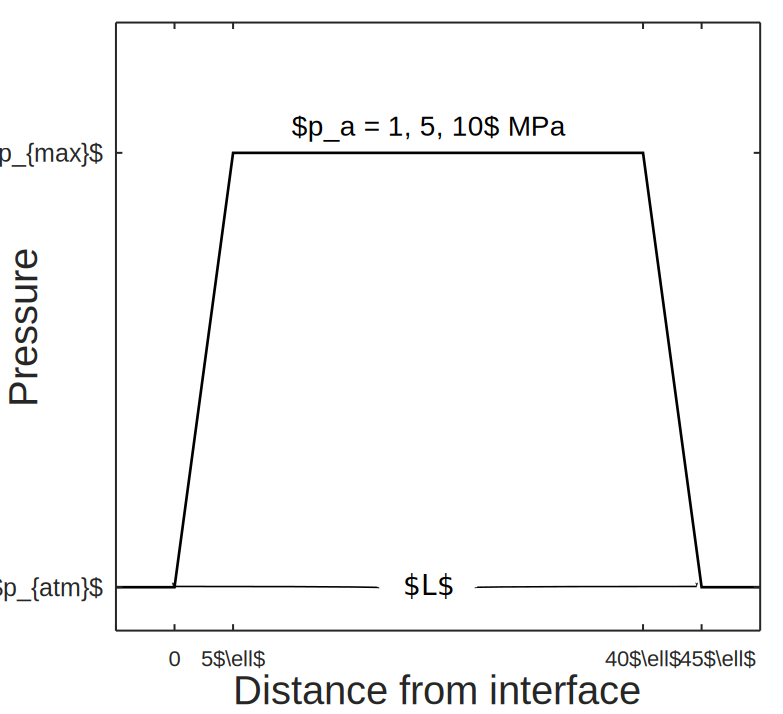
\includegraphics[width=0.5\textwidth]{./figs/lung_figs/p0_vs_y}
%   \caption{Initial pressure in the domain as a function of distance from the interface.}
%   \label{fig:p0_vs_y}
% \end{figure}

% We solve the dimensionless Euler equations of compressible, inviscid
% fluid motion in two dimensions ($x,y$),
% \begin{subequations} \label{eq:euler}
%   \begin{align} 
%     \frac{\partial \rho}{\partial t} + \frac{\partial \left(\rho u\right)}{\partial x} + \frac{\partial \left(\rho v\right)}{\partial y} = 0,\\
%     \frac{\partial \rho u}{\partial t} + \frac{\partial}{\partial x}\left( \rho u^2+p\right)  + \frac{\partial}{\partial y}\left( \rho uv\right) = 0,\\
%     \frac{\partial \rho v}{\partial t} + \frac{\partial}{\partial x}\left( \rho uv\right)  + \frac{\partial}{\partial y}\left( \rho v^2+p\right) = 0,\\
%     \frac{\partial E}{\partial t} + \frac{\partial}{\partial x}\left[u\left(E+p\right)\right] + \frac{\partial}{\partial y}\left[v\left(E+p\right)\right] = 0,
%   \end{align}
% \end{subequations}
% where $\rho$ is density, $p$ is the pressure, $u$ and $v$ are the
% velocity components in the $x$ and $y$ directions respectively, and
% $E$ is the total energy. We use the density and sound speed of air to
% nondimensionalize the system. To close the system, we use a stiffened
% equation of state which relate the total energy to the pressure and
% velocity in the flow, such that,
% \begin{align}\label{eq:stiffened_eos}
%   E=\frac{\rho\left(u^2+v^2\right)}{2} + \frac{p+\gamma B}{\gamma-1}.
% \end{align}
% Here $B$ is a measure of liquid stiffness. For perfect gases, such as
% is our treatment of air, $\gamma$ is the specific heats ratio and
% $B=0$. It is worth noting that the sound speed in our simulations is
% calculated based on the following relationship, derived from the
% stiffened equation of state.
% \begin{align}
%   c = \sqrt{\frac{\gamma\left(p+B\right)}{\rho}}
% \end{align}
% While physical diffusion is not considered in this setup, numerical
% diffusion does occur at fluid interfaces, creating a mixed region
% between the two fluids. To use a single equation of state, a mass
% fraction $Y$ is used to determine the material parameters
% ($\rho, \gamma, B, c$) of the mixed fluid such that $Y=1$ for pure
% water and $Y=0$ for pure air. Details of this implementation are
% explained by \cite{HenrydeFrahan2015} and additional mixture relations
% for properties can be found in \cite{Ward2010}. The
% dimensional and dimensionless values of each fluid property can be
% found in tables \ref{tab:usbe_lung_dimensional_parameters} and
% \ref{tab:usbe_lung_dimensionless_parameters} respectively.
% % 
% \begin{table}[htbp]%
%   \begin{center}
%     \caption{Dimensional properties of air and water used in simulations.}
%     \label{tab:usbe_lung_dimensional_parameters}%
%     \begin{tabularx}{0.75\textwidth}{| X | X | X | X | X |}
%       \hline
%       & Density, $\rho^*$ (kg/m$^3$) & $\gamma$ & $B^*$ (Pa)  & $c^*$ (m/s) ($p$=$1$ atm) \\ \hline
%       Air   & 1.1765                        & 1.4      & 0         & 347.23     \\ \hline
%       Water & 996                           & 5.5      & 492115000 & 1648.7     \\ \hline
%       \multicolumn{5}{l}{\small $^*$ indicates dimensional parameter}
%     \end{tabularx}
%   \end{center}
% \end{table}%
% \begin{table}[htbp]%
%   \begin{center}
%     \caption{Dimensionless properties of air and water used in simulations.}
%     \label{tab:usbe_lung_dimensionless_parameters}%
%     \begin{tabularx}{0.75\textwidth}{| X | X | X | X | X |}
%       \hline
%       & Density, $\rho$ & $\gamma$ & $B$ & $c$ \\ \hline
%       Air   & 1                          & 1.4      & 0         & 1          \\ \hline
%       Water & 846.6                      & 5.5      & 3469.1    & 4.75       \\ \hline
%       \multicolumn{5}{l}{\small Parameters are nondimensionalized by the density and sound speed of air. }
%     \end{tabularx}
%   \end{center}
% \end{table}

% To solve the governing equations, we implement a third-order accurate
% \ac{DG} scheme in space and a fourth-order accurate, adaptive
% Runge-Kutta method to march forward in time
% \citep{HenrydeFrahan2015}. A Rusanov approximate Riemann solver is
% used to compute the flux.  As previously stated, the computational
% domain width (x-direction) is $\lambda$. The domain length
% (y-direction) is 70$\lambda$. The grid resolution is 100 points per
% $\lambda$ unless otherwise stated. To minimize artificial reflections,
% inflow and outflow boundary conditions are used at the top and bottom
% of the domain, and the geometric grid stretching was implemented in
% the vertical direction for the top and bottom-most 10$\lambda$
% segments of the grid. Periodic boundary conditions are implemented at
% the left and right edges of the grid.


% \section{Analysis} \label{sec:usbe_lung_analysis} To answer the
% questions presented at the end of
% section \label{sec:usbe_lung_introduction}, we perform analysis to
% make some predictions about the vorticity and interface dynamics of
% the system to be solved. The results of this analysis are later
% compared to the results of our numerical results in section
% \ref{sec:usbe_lung_results} and discussed.

% \subsection{Vorticity generation order of magnitude analysis}
% We perform an order of magnitude analysis on each term of the
% vorticity generation equation for a 2D inviscid fluid
% system, 
% \begin{align} \label{eq:vorticity_euler}
%   \frac{\partial \vec{\omega}}{\partial t}+\left(\vec{u}\cdot\nabla\right)\vec{\omega} =% 
%   - \vec{\omega}\left(\nabla\cdot\vec{u}\right) + \frac{\nabla\rho\times\nabla p}{\rho^2}.%
% \end{align}
% Each of these terms represents a different physical mechanism by which
% the vorticity in the system is changing, with the terms on the left
% side of the equation representing changes in the existing vorticity
% field and the terms on the right representing vorticity sources and
% sinks. The first term on the left represents the total change of
% vorticity at any given point in the flow field. The second term on the
% left represents the advection of vorticity within the field. The first
% term on the right describes stretching of vorticity due to
% compressibility in the flow. And the last term on the right is the
% baroclinic term which represents vorticity generated by the
% misalignment of the pressure and density gradients in the flow. For
% our setup, we expect this to be governed by the pressure gradient of
% the acoustic wave and density gradient across the pertubed interface
% at points where the two meet obliquely.

% To perform the analysis, we specifically we consider the period in
% which the incoming compression wave is encountering the interface. It
% is assumed that the interface is static an undeformed from its
% initial state.



% As the above analysis suggests that circulation initially deposited by
% the compression wave is predominantly baroclinically generated we
% predict that circulation deposited will increase linearly with maximum
% acoustic pressure $p_a$, i.e.,
% $\Gamma \sim \frac{\nabla \rho\times\nabla p}{\rho^2}\sim p_a$.

% To numerically verify this prediction, we start from the vorticity generation equation for a 2D compressible, inviscid fluid.
% \begin{align} \label{eq:vorticity_euler}
%   \frac{\partial \vec{\omega}}{\partial t}+\left(\vec{u}\cdot\nabla\right)\vec{\omega} =% 
%   - \vec{\omega}\left(\nabla\cdot\vec{u}\right) + \frac{\nabla\rho\times\nabla p}{\rho^2}%
% \end{align}

% To determine the relative contributions to the half-domain circulation
% at each point in time we break the equation down into its individual
% component terms and integrate each over the right half domain. Doing
% this we arrive at the following set of equations,

% \begin{align}
%   \left(\frac{d\Gamma}{dt}\right)_{total} = \left(\frac{d\Gamma}{dt}\right)_{compressible} + \left(\frac{d\Gamma}{dt}\right)_{baroclinic} - \left(\frac{d\Gamma}{dt}\right)_{advective},
% \end{align}

% where 

% \begin{align}
%   &\left(\frac{d\Gamma}{dt}\right)_{compressible} &=& -\int_{A_R} \vec{\omega}\left(\nabla\cdot\vec{u}\right) \, dA_R,&\\
%   &\left(\frac{d\Gamma}{dt}\right)_{baroclinic} &=& +\int_{A_R} \frac{\nabla\rho\times\nabla p}{\rho^2}, dA_R,&\\
%   &\left(\frac{d\Gamma}{dt}\right)_{advective} &=& +\int_{A_R} \left(\vec{u}\cdot\nabla\right)\vec{\omega} \, dA_R,&
% \end{align}

% If the interface deformation after the wave has left the domain is
% entirely due to circulation, we expect from dimensional analysis that
% the interface amplitude will grow according to
% $a(t)/a_0 \sim \sqrt{\Gamma t}$.


% \section{Results and discussion} \label{sec:usbe_lung_results} Figure
% \ref{fig:trapz10_circ_interface} shows the early-time interface
% amplitude and half-domain circulation histories for the 10 MPa
% trapezoidal wave impinging on the water-air interface.

% \begin{figure}[h] 
%   \centering
%   \includegraphics[width=0.48\textwidth]{./figs/lung_figs/trapz10_intf_schematic}
%   \includegraphics[width=0.48\textwidth]{./figs/lung_figs/trapz10_circ_schematic}
%   \caption{The interface amplitude (left) and circulation (right)
%     histories corresponding to the $10$ MPa trapezoidal waves are shown
%     for $t\leq25$. Indicated times, $t_{1-4}$, are the times at which
%     different stages of the incoming pressure wave shown in Figure
%     \ref{fig:p0_vs_y} first encounter the interface.}
%   \label{fig:trapz10_circ_interface}
% \end{figure}

% Figure \ref{fig:trapz_circ_interface} shows the interface amplitude
% and half-domain circulation histories for 0$\leq t\leq$ 500 as
% functions of time for 1, 5, and 10 MPa amplitude trapezoidal
% waves impinging on the interface. The interface amplitude is plotted
% on logarithmically-scaled axes. 

% \begin{figure}[h] 
%   \centering
%   \includegraphics[width=0.48\textwidth]{./figs/lung_figs/interface_multi-amp_early}
%   \includegraphics[width=0.48\textwidth]{./figs/lung_figs/circulation_multi-amp_early}
%   \caption{The interface amplitude (left) and circulation (right) histories corresponding to the $1$(blue), $5$(orange), and $10$(yellow) MPa trapezoidal waves are shown for $t\leq 25$. The circulation history is normalized by the acoustic amplitude of the incoming wave to illustrate that circulation deposition scales linearly with $p_a$ \hl{(Update plot for Rusinov solver results)} }
%   \label{fig:trapz_circ_interface_early}
% \end{figure}

% \begin{figure}[h] 
%   \centering
%   \includegraphics[width=0.48\textwidth]{./figs/lung_figs/interface_multi-amp_loglog}
%   \includegraphics[width=0.48\textwidth]{./figs/lung_figs/circulation_multi-amp2}
%   \caption{The interface amplitude (left) and circulation (right) histories corresponding to the $5$(orange) and $10$(yellow) MPa trapezoidal waves are shown for $t\leq 500$. \hl{(Update plot for Rusinov solver results)}}
%   \label{fig:trapz_circ_interface_loglog}
% \end{figure}

% \begin{figure}[h] 
%   \centering
%   \includegraphics[width=0.48\textwidth]{./figs/lung_figs/placeholder}
%   \caption{The time derivative of each term of the circulation generation equation is shown.}
%   \label{fig:trapz_ddt_circ}
% \end{figure}


% \subsection{To be added to discussion}
% \textcolor{red}{ For typical acoustic waves, the pressure, velocity, and
%   density return to ambient conditions after the passing of the
%   wave. This implies that given a continuous acoustic waveform, the
%   integral the pressure gradient of over the entirety of the waveform
%   will be zero.  Hence if this wave interacts with a non-deforming
%   interface, the net baroclinic circulation deposited will be zero
%   \hl{(Must this be true if the wave itself is deforming during
%     interaction with the interface? I think so)}. Hence for an acoustic
%   wave to deposit net baroclinic circulation upon an interface, the
%   interface itself must deform during interaction with the wave. This
%   deformation alters the misalignment of the pressure and density
%   gradients at the interface, allowing for positive and negative
%   circulation deposited to not cancel out entirely. \hl{(Consider how
%     well the pressure gradient argument works in higher dimensions than
%     1. How does the direction of that pressure gradient change, relative
%     to the density gradient in 2D, 3D?)}  Note that this is not the case
%   for a shock wave, as the fluid need not return to ambient conditions
%   after the waves passing.}


% \section{Conclusions} \label{sec:usbe_lung_conclusions}

% \section{Future Work} \label{sec:usbe_lung_future}
% There are still many tasks and questions left to be investigated.

% \begin{itemize}
% \item Can we predict the amount of circulation deposited by a given wave?
% \item How would alveolar walls change the dynamics (thin layer of water on the side)?
% \item What is causing late time circulation growth?
% \item Why is the the Roe flux solver generating less circulation than the Rusinov?
% \end{itemize}

%%% Local Variables:
%%% mode: latex
%%% TeX-master: "../../prelim"
%%% End:
